%% LyX 2.0.1 created this file.  For more info, see http://www.lyx.org/.
%% Do not edit unless you really know what you are doing.
\documentclass[12pt,a4paper,twoside]{article}
%\usepackage{fontspec}
%\setmainfont[Mapping=tex-text]{Times New Roman}
\usepackage{color}
\usepackage{float}
\usepackage{url}
\usepackage{graphicx}
\usepackage{setspace}
%\onehalfspacing

\makeatletter

%%%%%%%%%%%%%%%%%%%%%%%%%%%%%% LyX specific LaTeX commands.
%\pdfpageheight\paperheight
%\pdfpagewidth\paperwidth

%% Because html converters don't know tabularnewline
%\providecommand{\tabularnewline}{\\}

%%%%%%%%%%%%%%%%%%%%%%%%%%%%%% User specified LaTeX commands.
\usepackage[left=25mm,right=25mm,top=28mm,bottom=20mm,headsep=4mm,footskip=8mm,voffset=-4mm]{geometry}
\usepackage{fancyhdr} %页眉页脚
\usepackage[square,super,comma,sort]{natbib} %文献格式
\usepackage{titletoc}
\usepackage{titlesec,amsmath}
%\usepackage[dvipsnames,svgnames,x11names]{xcolor} %彩色工具
\usepackage{xcolor}
\usepackage[bookmarks=true,bookmarksnumbered=false,colorlinks,linkcolor=black,citecolor=black,urlcolor=black]{hyperref}
\usepackage{booktabs}
\usepackage{subfigure}
\usepackage{graphicx}
%首行缩进
\parindent=2em
%% 定义正文字体
\usepackage{fontspec}
%\usepackage[slantfont,boldfont]{xeCJK}
\usepackage[BoldFont,CJKnumber]{xeCJK}
\setmainfont{Times New Roman}
\setmonofont{Consolas}
%\setmonofont{Courier New}
\setCJKmainfont{Adobe 宋体 Std}
\setCJKfamilyfont{song}{Adobe 宋体 Std}
\setCJKfamilyfont{hei}{Adobe 黑体 Std}
\newcommand\song{\CJKfamily{song}}
\newcommand\hei{\CJKfamily{hei}}

\renewcommand{\baselinestretch}{1.25}
\usepackage{xunicode}% provides unicode character macros
\usepackage{xltxtra} % provides some fixes/extras


% 重定义字号命令
\newcommand{\xiaochu}{\fontsize{30pt}{40pt}\selectfont}    % 小初, 1.5倍行距
\newcommand{\yihao}{\fontsize{26pt}{36pt}\selectfont}    % 一号, 1.4倍行距
\newcommand{\erhao}{\fontsize{22pt}{28pt}\selectfont}    % 二号, 1.25倍行距
\newcommand{\xiaoer}{\fontsize{18pt}{18pt}\selectfont}    % 小二, 单倍行距
\newcommand{\sanhao}{\fontsize{16pt}{24pt}\selectfont}    % 三号, 1.5倍行距
\newcommand{\xiaosan}{\fontsize{15pt}{22pt}\selectfont}    % 小三, 1.5倍行距
\newcommand{\sihao}{\fontsize{14pt}{21pt}\selectfont}    % 四号, 1.5倍行距
\newcommand{\banxiaosi}{\fontsize{13pt}{19.5pt}\selectfont}    % 半小四, 1.5倍行距
\newcommand{\xiaosi}{\fontsize{12pt}{15pt}\selectfont}    % 小四, 1.25倍行距
\newcommand{\dawuhao}{\fontsize{11pt}{11pt}\selectfont}    % 大五号, 单倍行距
\newcommand{\wuhao}{\fontsize{10.5pt}{10.5pt}\selectfont}    % 五号, 单倍行距
\newcommand{\xiaowu}{\fontsize{9pt}{9pt}\selectfont}    % 小五号, 单倍行距


%\renewcommand{\title}[1]{\def\ECUST@title{#1}}
%\def\ECUST@title{}
   
   \pagestyle{fancy}
   \renewcommand{\sectionmark}[1]{\markboth{#1}{}}
    \fancyhead[LO,RE]{\xiaowu{\leftmark}}%
    \fancyhead[RO,LE]{}%
%    \fancyfoot[LO,RE]{}%
%   \fancyfoot[LC,RC]{\thepage}
%  \fancyfoot[RO,LE]{}

\renewcommand{\contentsname}{\hei\erhao 目\quad 录}
\setcounter{tocdepth}{2}\setcounter{secnumdepth}{4}
\titlecontents{section}[18bp]{\vspace{0pt}}
    {\hei\xiaosan}{}
    {\hspace{.5em}\titlerule*[10pt]{$\cdot$}\contentspage}
\titlecontents{subsection}[14bp]{\vspace{0pt}}
    {\hei\sihao\quad}{}
    {\hspace{.5em}\titlerule*[10pt]{$\cdot$}\contentspage}

\renewcommand{\maketitle}{%
    \begin{center}%
%    {\bfseries\hei \xiaoer \ECUST@title}%
 %   {\bfseries\hei\xiaoer 面板数据模型的非参数回归估计及其R语言实现和应用}
    \\[0bp]%
    \end{center}%
}

\renewcommand{\thesubsection}{\Roman{subsection}}
\renewcommand{\thesubsubsection}{\arabic{subsubsection}}

%% 正文标题格式
\titleformat{\section}[hang]{\centering\hei\fontsize{17pt}{17pt}\selectfont}{}{1em}{}
\titleformat{\subsection}[hang]{\hei\xiaosan}{\thesubsection}{0.5em}{}
\titleformat{\subsubsection}[hang]{\bfseries\song\xiaosi}{\thesubsubsection}{0.5em}{}
\titlespacing{\section}{0bp}{12bp}{12bp}
\titlespacing{\subsection}{0bp}{12bp}{8bp}
\titlespacing{\subsubsection}{0bp}{12bp}{0bp}
   
% 图表定义
\renewcommand{\figurename}{\song \xiaowu 图}
%\numberwithin{figure}{section}
\renewcommand{\tablename}{\song \xiaowu  表}
%\numberwithin{table}{section}
%\renewcommand{\thefigure}{\thesection-\arabic{figure}}
%\renewcommand{\thetable}{\thesection.\arabic{table}}
%\makeatletter
%\@addtoreset{figure}{section}
%\makeatother


%公式按章编号
\numberwithin{equation}{section}
\renewcommand{\theequation}{\thesection-\arabic{equation}} 



%% 引用文献格式
%\let\textcite=\cite
%\renewcommand{\cite}[1]{\textsuperscript{\xiaosihao\textcite{#1}}}
\renewcommand\refname{\vspace{0pt}参考文献\vspace{12pt}}

%% 中文摘要和关键词


%一些行距
\makeatletter
\def\enumerate{%
 \ifnum \@enumdepth >\thr@@\@toodeep\else
   \advance\@enumdepth\@ne
   \edef\@enumctr{enum\romannumeral\the\@enumdepth}%
     \expandafter
     \list
       \csname label\@enumctr\endcsname
       {\usecounter\@enumctr\def\makelabel##1{\hss\llap{##1}}%
         \addtolength{\parsep}{0.25ex}
         \addtolength{\itemsep}{-8pt} %%%%
         \addtolength{\topsep}{-8pt}
         }
 \fi}
\makeatother

\makeatletter
\def\itemize{%
 \ifnum \@itemdepth >\thr@@\@toodeep\else
   \advance\@itemdepth\@ne
   \edef\@itemitem{labelitem\romannumeral\the\@itemdepth}%
   \expandafter
   \list
     \csname\@itemitem\endcsname
     {\def\makelabel##1{\hss\llap{##1}}%
         \addtolength{\parsep}{0.25ex}
         \addtolength{\itemsep}{-8pt} %%%%
         \addtolength{\topsep}{-8pt}
         } %%%%
 \fi}
\makeatother


\renewcommand\arraystretch{1.6}

\makeatother

\usepackage{xunicode}
\begin{document}
\thispagestyle{empty}

\begin{center}
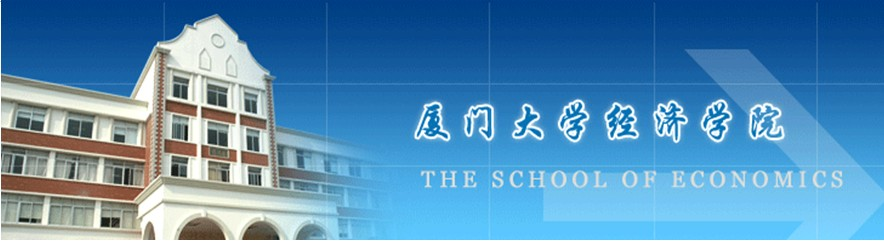
\includegraphics[width=16cm]{figure/jy}
\par\end{center}

厦门大学经济学院渊源于$1921$年建校初期的商学部。$1949$年以后,在厦门大学前校长、著名经济学家王亚南先生的带领和精心培育下,厦门大学经济学科得到了迅速发展。$1982$年$5$月经教育部批准,原厦门大学经济系升格为厦门大学经济学院,这是中国大陆重点综合性大学建立的第一所经济学院。$20$多年来,该院一直是中国大陆最重要的经济学教学与科研基地之一。

厦门大学经济学院是厦门大学规模最大的学院。现有经济学系、统计系、财政系、金融系、国际经济与贸易系和经济研究所、宏观经济研究中心、中国能源经济研究中心等$8$个教学科研单位,并设有教学实验中心。学院还拥有1个国家经济学基础人才培养基地,$1$个教育部人文社科重点研究基地,$1$个国家实验教学示范中心。

$2007$年经教育部批准,厦门大学经济学院的理论经济学和应用经济学被评为一级学科国家重点学科。其财政学、统计学、金融学、政治经济学、世界经济$5$个二级学科国家重点学科在国内具有重大影响,国际贸易学、西方经济学、劳动经济学、区域经济学、数量经济学、产业经济学等也具有较强实力。学院设有应用经济学和理论经济学$2$个博士后流动站,$11$个本科专业,$32$个硕士专业,$29$个博士专业。

厦门大学经济学院的教学科研条件优良,学术气氛浓厚,学术交流广泛,学院积极开拓和发展对外学术交流与合作,先后与欧美、日本、澳大利亚、新加坡及港、澳、台地区院校建立各种形式的学术交流和协作关系。

厦门大学经济学院的建设目标是加强现有优势学科的建设,加快经济学教学科研的现代化及国际化步伐,尽快建成国内一流,国际知名的经济学教学、研究基地。 

\begin{center}
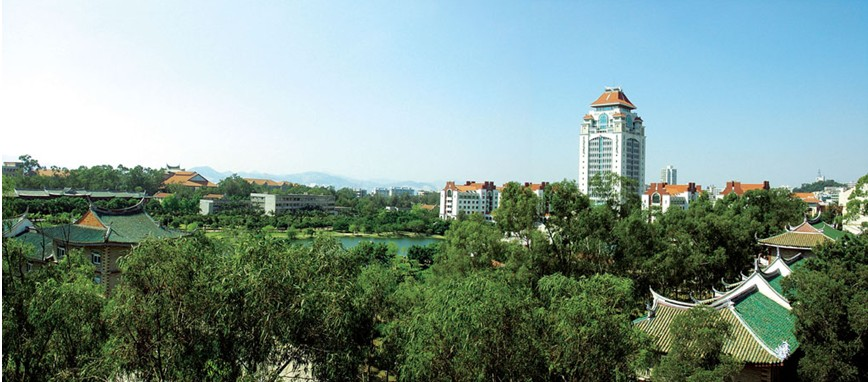
\includegraphics[width=16cm]{figure/xd}
\par\end{center}

\newpage{}

\thispagestyle{empty}

\tableofcontents{}

\newpage{}

\setcounter{page}{1}


\section{厦门大学统计系简介}

厦门大学计划统计系%
\footnote{\textcolor{black}{$2011$年$7$月$19$日计划统计系更名为统计系。}%
}由著名经济学家王亚南先生等创办于$1950$年,现已发展成为国内具有相当影响的统计、信息、投资分析类教学科研和人才培养基地。其学科和专业设置结构完整,包括统计学、国民经济学、数量经济学和经济信息管理学四个博士点(均可招收博士后)与四个硕士点,以及统计学(包括经济管理统计和投资决策分析两个方向)、信息管理与信息系统两个本科专业。所属的“厦门大学国民经济与核算研究所”由钱伯海先生创办于$198$3年,是国内最早建立的国民核算专门研究机构,先后承担多项国家社科基金、自然科学基金重点科研项目。鉴于各方面成就,其统计学科分别于$1987$年、$2001$年和$2007$年连续三次被国家教委和教育部评为国家级重点学科。厦门大学统计学科于$2008$年经教育部批准,厦门大学统计学教学团队被教育部评为国家级教学团队,统计学专业被评为国家级特色专业。$2008$年,国家统计局批准在厦门大学设立“国家统计局统计科学研究所研究基地”。在教育部和厦门大学的指导下,经过本学科全体成员的共同努力,现已建设成为国内具有重要影响和代表性的统计人才培养基地和学术研究基地。

全系教师通过长期探索和反复实践,积累了丰硕的科研和教学成果,在统计理论方法和国民经济核算这两个领域尤为突出。近年来,其教学科研正不断向现代统计方法及其应用、可持续发展统计和环境经济核算、经济计量和时间序列分析、实验经济学、投资决策分析、数据挖掘、经济信息管理等前沿领域拓展。统计系承担了多项国家社科基金重点科研项目,以及国家自然科学基金和其他省部级科研项目,有关研究成果曾多次获得国家级和省部级奖励。

六十年来,厦门大学计划统计系已培养本科层次的专门人才二千多人,博士和硕士层次的高级专门人才五百多人。他们在各行各业发挥着自己的聪明才智,为母校和母系赢得了荣誉,其中在数量方面的特色,为国内金融市场、房地产市场输送了大量人才。 

\newpage{}


\section{厦门大学数据挖掘研究中心(DMRC)简介}

\begin{spacing}{1.2}
厦门大学数据挖掘研究中心(Data Mining Research Center,DMRC)组建于$2006$年,于$2010$年$7$月由厦门大学校长工作会议决议通过并正式成立,成为厦门大学直属的教学科研机构。在厦门大学各级领导的关心和支持下,由辅仁大学谢邦昌教授、厦门大学朱建平教授和美国耶鲁大学马双鸽教授联袂携领,中心从最初$20$余人的学习小组逐渐发展成为国内具有一定影响力的学术研究机构。同时中心陆续聘请美国工程院院士吴建福教授、美国得克萨斯农机大学吴曦明教授、美国宾州州立大学林共进教授、美国雪城大学陈江教授等$20$多名国内外著名学者组成中心顾问委员会。为更好地学习社会实践和服务社会,中心还聘请了中海油首席经济学家邱晓华博士、澳门前诚兴银行董事长禤永明先生、厦门银行副行长陈锋博士、福建华通工商资讯有限公司徐积章总经理等各界精英。

厦门大学数据挖掘研究中心依托厦门大学经济学院统计系,充分发挥学科交叉优势,是在整合统计学、计量经济学、数量经济学、信息管理学等相关学科基础上成立的跨学科、综合型、开放式的教学研究机构。目前中心下设数据挖掘与商业智能研究所、社会调查与数据分析研究所、金融计量与投资决策研究所、生物信息分析研究所、社会服务办公室等五个部门,充分发挥中心在科学研究、人才培养、学术交流和资料信息建设、社会调查与咨询服务、商业智能与数据挖掘服务、云端计算开发等各个领域的优势力量。
中心一贯注重教学工作,努力提高学生素质,致力于培养专业化、创新型人才。同学们可以结合自己的兴趣选择参加数据挖掘基础、高级数据挖掘原理与技术、数据挖掘产业应用实务等三个讨论班,同时充分借助来自耶鲁大学、美国得克萨斯农机大学和宾州州立大学等顶级名校专家委员的智力支持。

自组建以来,中心脚踏实地,成绩斐然。在老师与同学们的共同努力下,举办了“国际金融数据挖掘研讨会”、“统计学的最新进展与挑战国际研讨会”等多个国内外重要统计学学术会议;承担$30$多项国家级、省部级课题以及企事业横向课题,内容涵盖金融风险、数据挖掘、数据质量管理、经济系统预警及指数指标体系等多个方面。在《Annals
of Statistics》、《Biostatistics》、《Statistics in Medicine》、《Nonparametric
Statistics》、《Communication in Statistics》、《Annals of Operation Research》等国际权威期刊发表$20$多篇。同时,在《经济研究》、《经济学动态》、《统计研究》、《数理统计与管理》等国内经济统计学权威期刊发表文章$50$多篇,完成数部专著。

借助已逐步形成的教学科研软实力,中心已经构建起一支专门从事数据挖掘研究、特色鲜明、具有核心竞争力的学术创新团队。特别值得一提的是,中心举办的“海西金融、旅游、消费信心指数发布会”已成为中心标志性品牌,在社会上引起强烈反响。自$2009$年以来,中心发布的季度指数信息被新华社、光明日报、中央人民广播电台、厦门日报等各大媒体以及网易、新浪网、华夏经纬网、中新网等$80$多家网络媒体发布、转载,逐渐成为帮助政府和社会大众准确掌握社会经济现状的风向标,对于推进福建扩大开放、促进海峡西岸经济社会协调发展具有重要的现实作用和深远的战略意义。

过往的成绩是我们不断进步的基石,未来的憧憬是我们从不懈怠的动力。厦门大学数据挖掘研究中心将继续为推广新兴数据挖掘技术,提高国内企业机构的商业智能水平而努力,进一步扩大厦门大学统计系和数据挖掘研究中心在全国范围内的知名度和影响力,使中心逐步成为全国统计学、数据挖掘研究重镇和人才培养的重要基地。
\end{spacing}

\newpage{}


\section{厦门银行:向一流的区域银行进军}

$1996$年$11$月$30$日,厦门城市合作银行(厦门银行的前身)正式成立,厦门人的金融梦想由此开启。自成立以来,厦门银行秉承“创新金融,服务社会;创设平台,成就员工;创造价值,回报股东”的历史使命,践行“心手相连,承诺百年”的服务理念,坚持“服务地方经济、服务中小企业、服务台商、服务市民”的市场定位,在社会各界的关心和支持下,锐意进取、敢于创新,取得质量、效益、规模协调发展的良好成果。

近年来,厦门银行成功引入台资背景的战略投资者、圆满完成行名变更,服务区域从厦门延伸到海西的中心城市,以及台商聚集的国内其他城市等,实现了跨越发展的一个又一个辉煌,完成了从经营困难的城市信用社向富有朝气、极具成长性的商业银行的华丽转身。截至$2011$年底,厦门银行已陆续在福州、泉州、重庆等地设立分行;资产、负债、净利润均实现较快增长;不良贷款持续双降,风险抵御能力进一步增强。

近日,基本提前完成$2010\sim2012$年战略规划的厦门银行,正与该行聘请的国际知名战略管理咨询公司波士顿咨询公司(简称“BCG”)紧锣密鼓地制定未来$5$年战略规划,在最新的规划中,厦门银行首次提出要成为“立足海西、服务闽台、辐射全国、跻身一流区域银行”的战略愿景。

\begin{spacing}{0.90000000000000002}

\subsection*{先行先试,创新台商金融服务产品}
\end{spacing}

作为首家具有台资背景的商业银行,厦门银行充分利用战略投资者——富邦银行的管理支持和信息支持,在两岸金融合作上先行先试,为大陆台商、台北富邦银行及香港富邦银行客户在大陆的分支机构提供量身定制的融资以及便利的结算、现金管理等全方位的金融服务。

比如和台北富邦银行共同推出的“两岸通”美元速汇业务,为两岸三地企业与个人汇款业务提供便利;“内保外贷”业务,专为解决台商客户境外子公司海外融资难、借款利率高的难题而推出的产品;“外保内贷”
业务,针对台商客户大陆融资难的问题,通过母公司在台湾或境外银行申请额度开立担保信用证,厦门银行给予其在大陆子公司授信;“异地抵押贷款”业务,针对公司及股东资产在港台的大陆台资企业客户,以抵押其港台资产获取备用信用证的方式获取授信放款,有效解决境内台资企业的融资困扰;“新台币兑换业务”业务,该行$2010$年$12$月$31$日正式开办新台币兑换业务,成为获准开办新台币兑换业务为数不多的几家银行之一。

\begin{singlespace}

\subsection*{灵活高效,助力小微企业发展}
\end{singlespace}

早在$2006$年$4$月,厦门银行就成立了“中小企业主贷款中心”,$2009$年更是率先成立小企业信贷部,专门服务辖内的小微企业。在近年来信贷规模管控、中小企业融资难的情况下,厦门银行大力倾斜扶持小微企业业务,为小微企业过冬提供金融专案。近两年该行小企业贷款余额年均复合增长率约为$87\%$,且总体上呈加速增长态势。由于在服务中小企业方面积累了丰富的经验,厦门银行多次被中国银监会授予“小企业金融服务先进单位”荣誉称号。

针对企业不同的发展时期,厦门银行为其量身定做了专门的产品对应。比如,在企业的创业阶段,厦门银行推出了创业快速贷——个人助业贷款,向企业的法定代表人、股东等关键人提供用于企业日常经营周转的个人贷,最高$500$万元、最长$10$年;发展期的小企业可享有小企业担保贷款,这是由小企业固定资产抵押或第三方保证等担保的、用于企业日常经营周转的流动资金贷款,抵押率高、最长$10$年,还可异地房产抵押;步入正轨的、具有较高成长性的小企业可享有股东联保贷款,企业凭借股东信用向该行申请贷款,无须实物担保,即可根据信用评级获得相应金额的信用贷款。

截至$2011$年末,厦门银行中小企业人民币贷款余额占全行贷款余额的近$70\%$,余额增量占全行贷款增量的四分之三。今后,随着厦门银行继续贯彻落实加大对中小企业的支持力度,以上比例将持续提高。

\begin{singlespace}

\subsection*{增值服务,打造亲切的社区银行}
\end{singlespace}

“心手相连,承诺百年”是厦门银行的服务理念。厦门银行不仅要为客户创造良好的环境,提供用心贴心的服务,还积极为客户提供可持续增值的服务。作为目前城商行中开展零售业务种类最为丰富的银行之一,厦门银行将提供凤凰花理财、黄金投资交易、凤凰花理财卡等可持续增值的个人金融服务产品。

“凤凰花”理财产品历来以收益率高、风险低、品种多而广受客户赞誉;作为上海黄金交易所金融类会员、国内少数能同时接受法人与个人客户委托的银行之一,厦门银行黄金交易的品种丰富,既有现货交易,又有延期交收交易,$2010$年还荣登“中国黄金投资行业顾客满意十佳诚信企业”。凤凰花理财卡则通过系统化的业务关联和个性化的业务服务,整合客户各项投资理财需求,打造超值服务的综合理财卡。

自立行以来,厦门银行一直致力于成为街坊邻里喜爱的社区银行,该行借鉴富邦银行的先进经验,通过社区化、专属化、便利化的服务模式,为广大市民提供集存款、贷款、理财、投资为一体的全方位金融体验,获得了街坊邻里的一致好评。

\begin{singlespace}

\subsection*{热心公益,积极承担社会责任}
\end{singlespace}

$3$月$14$日晚,在厦门大学科学艺术中心,厦门大学与厦门银行共同举办了一场“世界经典声乐作品音乐会”。知名女中音歌唱家毕宝仪女士、美国男中音歌唱家达蒙·普鲁密斯和德国青年钢琴演奏家卡罗琳娜·特洛约克等音乐家为厦大师生与厦门银行邀请的高端客户带来了声乐套曲《吉普赛人之歌》、歌剧《灰姑娘》、歌剧《唐璜》二重唱、歌剧《魔笛》以及俄罗斯民歌等世界音乐经典曲目。

近年来,厦门银行正处于快速发展的阶段,在抓管理、抓业绩的同时,厦门银行积极践行“创新金融,服务社会”的历史使命,主动承担与履行社会责任,积极支持地方教育、文化等事业的发展,$2010$年投入$200$万元大力赞助“闽南神韵”项目、参与赞助海峡音乐节活动等。与此同时,该行十数年如一日地积极支持社会公益活动,常年在营业网点设置慈善捐款箱,号召员工进行慈善一日捐,帮助市慈善总会募集善款;积极参与无偿献血活动,组织全体员工向汶川地震、青海玉树地震、舟曲泥石流、省内洪涝地区捐款等。$2011$年,厦门银行还一次性向厦门市老年基金会捐款$100$万元,用于救助厦门市有困难的老年弱势群体。 

\newpage{}


\section{海西金融、旅游、消费信心指数介绍}

消费者信心指数是对消费者消费心理感受变化的测度,它是通过居民住户调查搜集资料,采用一定的统计方法计算得到的反映消费者信心变动程度的指标,是综合反映并量化消费者对当前经济形势评价和对经济前景、收入水平、收入预期以及消费心理状态的主观感受,也是预测经济走势和消费趋向的一个先行指标。通俗地说,通过观察这一指数的高低和趋势,可以清晰判断居民的消费开支意愿变化和对未来经济的乐观程度。在西方经济成熟国家,消费者信心指数的重要性绝不会亚于CPI和就业率指标。每逢该数据公布前期,往往市场就会形成静默等待的气氛。一旦数据出炉,市场往往会根据之前预测情况的高低变化,迅速做出反应。

$2011$年是“十二五”规划的开局之年,受惠于国务院$2009$年$5$月和$2011$年$4$月先后颁布了《关于支持福建省加快建设海峡西岸经济区的若干意见》和《海峡西岸经济区发展规划》,海峡西岸经济区步入了崭新的发展阶段。在新的起点上加快建设海峡西岸经济区,必须增强信心,把保持经济平稳较快发展和加快经济发展方式转变有机统一起来。一般情况下,(金融、旅游、消费)信心指数可以一定程度上反映公众对宏观经济主要问题的信心水平和前景预期,可作为预测经济走势和消费倾向的一个先行指标。因此,发布金融、旅游、消费信心指数具有较强的实践价值和政策意义。温家宝总理在不同场合曾多次强调过信心的重要性,在$2011$年$3$月$14$日答中外记者问时,总理再次提及信心:“我们要有忧患意识,始终保持清醒的头脑。同时,又要树立信心,信心就像太阳一样,充满光明和希望。”

$2009$年,厦门大学计划统计系和厦门大学数据挖掘研究中心成功发布厦门市金融、旅游、消费信心指数,受到了香港文汇报、福建日报、光明网、新浪网、新华网、中新网、光明日报等多家媒体报道,取得了强烈的社会效应。$2010$年初,本着进一步支持海峡西岸经济区建设和为政府、企业提供决策参考的意识,厦门大学经济学院计划统计系、厦门大学数据挖掘研究中心课题组策划了海西消费信心指数调查,将调查范围由厦门扩展至海峡西岸经济区,涵盖福建(福州、厦门、泉州、漳州、龙岩、莆田、三明、南平、宁德)以及福建周边省份:浙江(温州、丽水、衢州、台州、金华)、江西(上饶、鹰潭、抚州、赣州)、广东(梅州、潮州、汕头、汕尾、揭阳)等,共计$23$个城市。

海西金融、旅游、消费信心指数调查在厦门大学社科处的支持下,在厦门大学经济学院副院长、统计系曾五一教授领导下,由厦门大学经济学院统计系朱建平教授、厦门大学经济学院统计系讲座教授、辅仁大学统计资讯系谢邦昌教授负责规划分析,由厦门大学数据挖掘中心与厦门银行股份有限公司联合组成的课题组以及厦门大学经济与管理实验教学中心开展实施,包括前期文献查阅、方案设计、访员培训、电话访问、数据分析、调查报告的撰写及指数发布,具体调查工作由北京商智通信息技术有限公司协助完成。调查采用雅典娜电话调查系统(AthenaCATI)以电脑随机抽样的方式对海西经济区$20$岁以上居民进行调查。


\subsection*{海西概况}

海峡西岸经济区,简称“海西”,是指台湾海峡西岸,以福建为主体包括周边地区,南北与珠三角、长三角两个经济区衔接,东与台湾岛、西与江西的广大内陆腹地贯通,具有对台工作、统一祖国,并进一步带动全国经济走向世界的特点和独特优势的地域经济综合体。它是一个涵盖经济、政治、文化、社会等各个领域的综合性概念,总的目标任务是“对外开放、协调发展、全面繁荣”,基本要求是经济一体化、投资贸易自由化、宏观政策统一化、产业高级化、区域城镇化、社会文明化。截止目前海峡西岸经济区包括福建周边的浙江温州、丽水、衢州、金华、台州;江西上饶、鹰潭、抚州、赣州;广东梅州、潮州、汕头、汕尾、揭阳以及福建福州、厦门、泉州、漳州、龙岩、莆田、三明、南平、宁德,共计23市。

\newpage{}


\section{2012年第一季度海西金融、旅游、消费信心指数新闻稿}


\section*{金融信心指数回暖,海西总体信心指数小幅上扬}

$4$月$27$日上午,厦门大学、辅仁大学、厦门银行股份有限公司在福州市西湖宾馆福建会堂厦门厅联合发布了由海峡两岸大学共同发起调查的“$2012$年第一季度海西金融、旅游、消费信心指数”。此次调查由厦门大学、辅仁大学、厦门银行股份有限公司联合主办,厦门大学数据挖掘研究中心、厦门大学经济学院统计系、辅仁大学管理学院、北京商智通信息技术有限公司、厦门大学经济与管理教学实验中心联合承办。调查采用北京商智通雅典娜电话调查系统(AthenaCATI)以电脑随机抽样方式进行,调查样本涉及海西$23$个城市$4370$位$20$岁以上居民(其中包含$1329$份厦门市调查样本)。


\subsection*{海西信心总指数小幅上升,各分项指数表现各异}

调查结果显示,$2012$年第一季度海西金融、旅游、消费信心总指数为$92.81$点,较上一季度环比小幅上升$0.70$点,较去年第一季度同比回落$4.73$点。总指数得分在$100$点以下的悲观区间,表明海峡西岸大部分居民总体信心略显不足,这一预期与国家放缓经济增速的宏观调控政策相一致。消费者对经济形势的评价和经济发展中的诸多不确定因素仍持谨慎态度,而这也是居民理性选择的结果。

“海西金融、旅游、消费信心指数”自$2010$年第一季度以来,已经连续发布了$9$个季度。报告显示,本季度金融指数、旅游指数和消费指数中得分最高且唯一位于乐观区域的是旅游指数($110.18$)。当前国内旅游政策环境持续利好,节假日依然是主要拉动因素,海西居民不仅有较强的出行意愿,且对本地旅游收入也持有信心。

消费指数($94.42$)虽仍处于悲观区域,但自$2010$年第四季度以来首次出现小幅上涨,环比微扬$0.46$点。尽管$3$月份CPI短暂反弹至超预期的$3.6\%$,但是通货膨胀问题已在货币政策收紧和经济增速放缓的下拉力量中步步回落。海西消费者在提升消费信心的同时,也更趋向于保持理性、谨慎的态度。

本季度金融指数结束长期下降趋势,得分为$69.03$点,环比上升$2.78$点,同比略降$0.70$点,其中环比增幅最大的是福建省(环比上升$3.36$)。金融指数包括金融投资计划指数和金融投资比例指数,其中金融投资计划指数($62.10$)环比大幅回升$4.30$点,增幅为所有分项指数中最大。 


\subsection*{经济发展信心止跌回升,海西建设信心上扬}

调查结果显示,$2012$年第一季度海西地区经济发展信心指数为$95.30$点,环比上一季度提高$0.75$点,虽仍在中性偏向悲观区域,但已呈现探底回升趋势。从分项指数看,物价信心指数为$85.95$点,环比上季度上升$1.45$点,同比下降$6.15$点,虽仍陷于悲观区域,但已逐步企稳回升;经济景气指数为$104.65$点,环比上升$0.05$点。消费者信心的提升主要得益于“两会”精神鼓舞、“十二五”规划各项具体举措的陆续出台以及通货膨胀的持续回落。根据分省数据,福建经济发展信心指数$93.76$点,浙江$98.72$点,江西$94.65$点,广东$97.48$点。浙江和广东发展信心水平较高,相比之下福建和江西经济发展信心略显不足。

一季度海西建设信心指数为$98.00$点,环比上升$0.10$点,同比下降$10.70$点,仍旧处于略微悲观区域。继上个季度该指数($97.90$)两年来首次跌入悲观区域后,本季度指数有所回升。自去年以来,国务院相继批准发布了《海峡西岸经济区发展规划》和《平潭综合实验区总体发展规划》,国家对海西经济区发展的政策支持力度空前,海西民众对未来半年海西地区建设的信心正在恢复。 


\subsection*{耐用品投资信心回暖,就业信心小幅回升}

本季度海西地区耐用品投资状况指数为$85.50$点,处于悲观区域,较上个季度回升$0.87$点,呈探底回升之势,同比下降$6.63$点。其中,耐用品购买指数为$89.45$点,环比上升$0.60$点,同比下降$8.25$点。虽然耐用消费品投资信心仍处在低位,但是本季度央行两次下调存款准备金率,宽松的货币政策使得耐用消费品投资信心回暖。然而持续上行的油价对消费者购买汽车等造成一定负面影响,加之经济大环境持续低迷和政策的不确定性等因素也使消费者仍持观望和谨慎态度。房地产购买信心指数为$81.55$点,环比上升$1.15$点,同比回落$5.00$点。房地产调控政策已实施一年有余,调控成果持续显效,购房者信心有所提振,降价潮已经进入平稳期。但是目前市场对房价的敏感度依旧较高,海西消费者的购房信心仍不够强烈。

一季度,海西地区就业信心指数为$91.00$点,随着就业旺季的过去,就业形势日益趋紧,居民的就业主观预期较弱,但就业信心较上一季度略升$0.10$点,已出现好转迹象。从分省数据上看,海西四省就业信心水平中居首位的是福建省($92.21$),最低的省份是广东省($86.01$),所有省份就业信心指数均落在悲观区域。增加岗位,促进就业,成为海西各省市共同面对的问题。 


\subsection*{金融信心触底回升,旅游信心持续乐观}

金融信心指数($69.03$)的触底反弹成为本次海西信心指数的一大亮点。从外围环境看,欧债主权债务危机走出阴霾,美国经济稳步回升,美国等发达国家股市创出金融危机以来新高;从国内环境看,货币政策放松预期和中国A股市场一季度的反弹走势,各种因素的叠加引发了居民对国内金融环境的乐观预期,成为推动海西消费者信心上升的主要动力。一季度海西金融指数环比上升$2.78$点,达到$69.03$,尽管该指数依然落在悲观区域,但是金融投资计划指数在所有指数中环比增幅最大,有触底回升态势。

本季度海西旅游信心指数环比略降$0.42$点,尽管略有下降,但高达$110.18$点的乐观数值表明旅游信心仍处于稳步上升通道。经济环境的回暖、交通出行工具的日益完善以及人均收入的逐步增高均促进了旅游经济更上一层楼,日渐成为海西多个城市经济发展的重要支柱。从历次旅游信心指数来看,海西居民既有较强的出行意愿,又对本地旅游收入持有信心,随着国内经济走势日趋明朗,旅游信心指数将继续保持良性循环。



\newpage{}


\section{2012年第一季度海西金融、旅游、消费信心指数调查报告}


\subsection{引言}

“海峡西岸经济区”这一概念在$2004$年首次提出时就引发了社会各界不同凡响的关注,近年来国家对海西经济区建设的重视也不断升温。国务院$2009$年$5$月和$2011$年$4$月先后颁布了《关于支持福建省加快建设海峡西岸经济区的若干意见》和《海峡西岸经济区发展规划》,“十二五”规划纲要中更是两次提及海峡西岸经济区建设,并且独辟章节阐述“支持海峡西岸经济区建设”的具体任务与政策举措。然而建设海峡西岸经济区并非一蹴而就的易事,其中机遇与挑战并存,因此海西各界必须增强信心,明确海西建设的发展目标,不断细化加快海西建设的目标任务和政策举措。

在海西的建设过程中,民众的力量有着不可忽视的作用,民众的信心也关系到经济建设能否平稳快速的进行。一般情况下,(金融、旅游、消费)信心指数可以一定程度上反映公众对宏观经济主要问题的信心水平和前景预期,可作为预测经济走势和消费倾向的一个先行指标。因此,发布海西金融、旅游、消费信心指数具有较强的实践价值和政策意义。

$2009$年,厦门大学统计系和厦门大学数据挖掘研究中心成功发布厦门市金融、旅游、消费信心指数,受到了香港文汇报、福建日报、光明网、新浪网、新华网、中新网、光明日报等多家媒体报道,取得了强烈的社会效应。$2010$年初,本着进一步支持海峡西岸经济区建设和为政府、企业提供决策参考的意识,厦门大学经济学院统计系、厦门大学数据挖掘研究中心课题组策划了海西消费信心指数调查,将调查范围由厦门扩展至海峡西岸经济区,涵盖福建(福州、厦门、泉州、漳州、龙岩、莆田、三明、南平、宁德)以及福建周边省份:浙江(温州、丽水、衢州、台州、金华)、江西(上饶、鹰潭、抚州、赣州)、广东(梅州、潮州、汕头、汕尾、揭阳)等,共计$23$个城市
。

海西金融、旅游、消费信心指数调查在厦门大学社科处的支持下,在厦门大学经济学院副院长、统计系曾五一教授领导下,由厦门大学经济学院统计系朱建平教授、厦门大学经济学院统计系讲座教授、辅仁大学统计资讯系谢邦昌教授负责规划分析,由厦门大学统计系数据挖掘中心与厦门银行股份有限公司联合组成的课题组以及厦门大学经济与管理实验教学中心开展实施,包括前期文献查阅、方案设计、访员培训、电话访问、数据分析、调查报告的撰写及指数发布,具体调查工作由北京商智通信息技术有限公司协助完成。

本次调查采用雅典娜电话调查系统(AthenaCATI)以电脑随机抽样的方式对海西经济区$20$岁以上居民进行调查,是继$2010$年海西金融、旅游、消费信心指数调查之后的又一次全新的调查,同时是第$13$次厦门金融、旅游、消费信心指数调查及第$9$次海西金融、旅游、消费信心指数调查。

$2012$年第一季度调查共搜集到海西$23$个市$4370$份有效样本,其中包含$1329$份厦门调查样本。现借此次发布会发布海西$2012$年第一季度及厦门市$2012$年第一季度金融、旅游、消费信心指数调查结果并和$2011$年度的调查结果进行比较。

消费者信心指数采用扩散指数模型,指数结果介于$0$至$200$分之间,信心依指数值增加而递增,其中,若指数落在$0\sim100$之间,则偏向悲观;若指数落在$100\sim200$之间,则偏向乐观;以$100$表示中立水平。 


\subsection{海西指数综述}

本季度海西地区总指数$92.81$,较上季度上升$0.70$点,比去年同期下降$4.73$点。其中消费指数$94.42$,环比上升$0.46$点,同比下降$8.80$点;旅游指数$110.18$,环比微降$0.42$点,同比上升$7.55$点;金融指数$69.03$,环比上升$2.78$点,同比略降$0.70$点。


\subsection{海西分项指数分析}


\subsubsection{经济发展信心评析}

如图\ref{fig:=006D77=00897F=007ECF=006D4E=0053D1=005C55=004FE1=005FC3=006307=006570}所示,$2012$年第一季度海西地区经济发展信心指数$95.30$,与$2011$年第一季度相比,该指数同比下降$10.40$点,虽然该指数连续三个季度低于$100$,目前仍处于悲观区域,但是已呈探底回升趋势,环比上升$0.75$点。从分项指数来看,物价指数$85.95$,环比上升$1.45$点,同比下降$6.15$点,虽仍陷于悲观区域,但是逐步企稳回升;经济景气指数$104.65$,环比上升$0.05$点,同比降低$14.65$点。这一信号说明通胀水平的降低和“十二五”各项规划的陆续出台使海西居民对新一轮经济复苏的到来信心有所回升,但是$2012$年我国经济转型带来的经济增速放缓也使民众多一分谨慎,看法略微悲观,海西地区经济发展信心要恢复到$2011$年一季度的水平($105.70$),还需要一段时间。

\begin{figure}[H]
\begin{centering}
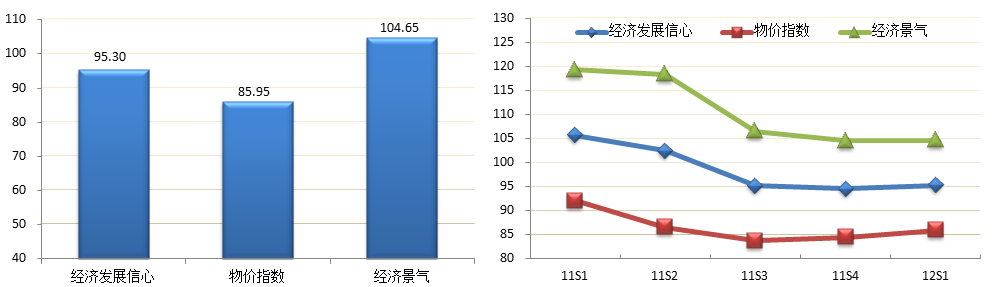
\includegraphics[width=16cm]{figure/海西经济发展信心指数}
\par\end{centering}

\centering{}\caption{\label{fig:=006D77=00897F=007ECF=006D4E=0053D1=005C55=004FE1=005FC3=006307=006570}海西经济发展信心指数}
\end{figure}


调查结果显示,从分省数据来看,福建经济发展信心指数$93.76$,浙江$98.72$,江西$94.65$,广东$97.48$,如图\ref{fig:=005404=007701=007ECF=006D4E=0053D1=005C55=004FE1=005FC3=006307=006570}所示。四省居民对未来半年的经济发展信心都处在悲观区域,从时间趋势(折线图)来看,浙江和广东发展信心水平较高,相比之下福建和江西经济发展信心略显不足,江西环比降低$0.38$点。

\begin{figure}[H]
\begin{centering}
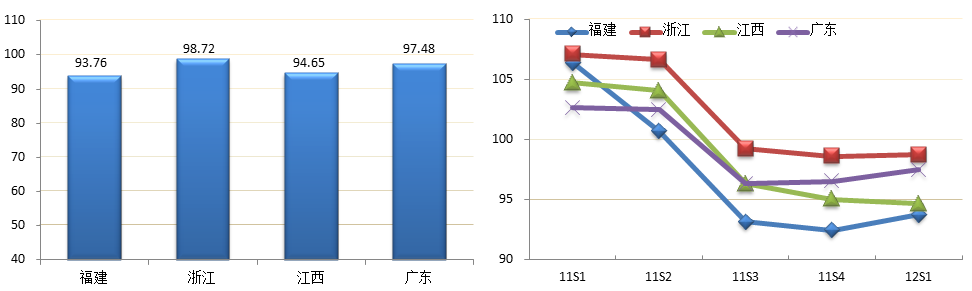
\includegraphics[width=16cm]{figure/各省经济发展信心指数}
\par\end{centering}

\centering{}\caption{\label{fig:=005404=007701=007ECF=006D4E=0053D1=005C55=004FE1=005FC3=006307=006570}各省经济发展信心指数}
\end{figure}



\subsubsection{家庭生活状况信心评析}

$2012$年第一季度海西地区生活状况指数$102.38$,比上季度略升$0.13$点,比去年同期下降$9.20$点,处于略微乐观水平。其中,分指标家庭经济状况指数$99.85$,环比微升$0.35$点,同比下降$10.45$点;家庭支出状况指数$104.90$,环比略降$0.10$点,同比下降$7.95$点,如图\ref{fig:=006D77=00897F=00751F=006D3B=0072B6=0051B5=004FE1=005FC3=006307=006570}所示。国家统计局公布的消费物价指数(CPI)显示,今年$1$月份CPI同比增长$4.5\%$,2月份CPI同比增长$3.2\%$,从去年下半年以来国家出台的各项控制通胀政策效果初显,通胀水平有所回落。今年,中央多次强调转变经济增长方式,让消费成为拉动经济增长的新引擎,海西居民对未来半年家庭支出状况的乐观程度将有利于扩大内需,但由于经济增速放缓,海西居民对未来半年家庭经济状况的改善持略微悲观态度。
\begin{figure}[H]
\begin{centering}
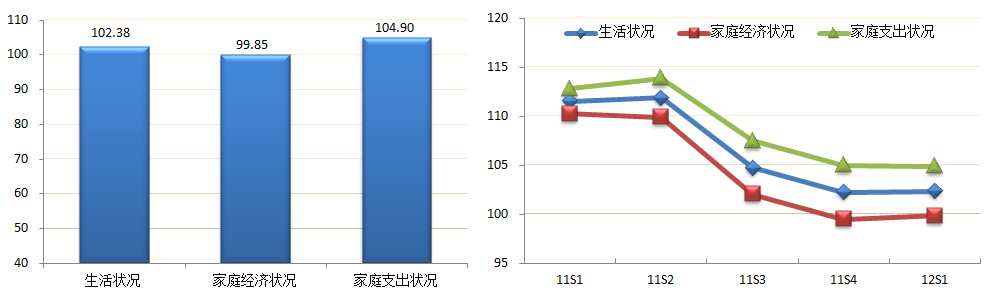
\includegraphics[width=16cm]{figure/海西生活状况信心指数}
\par\end{centering}

\centering{}\caption{\label{fig:=006D77=00897F=00751F=006D3B=0072B6=0051B5=004FE1=005FC3=006307=006570}海西生活状况信心指数}
\end{figure}


如图\ref{fig:=005404=007701=00751F=006D3B=0072B6=0051B5=004FE1=005FC3=006307=006570},分省数据显示,福建、浙江、江西、广东四省未来半年内生活状况信心均处于乐观区域,浙江的信心水平最高,生活状况信心指数为$102.99$,其次是福建,广东、江西位居其后。
\begin{figure}[H]
\begin{centering}
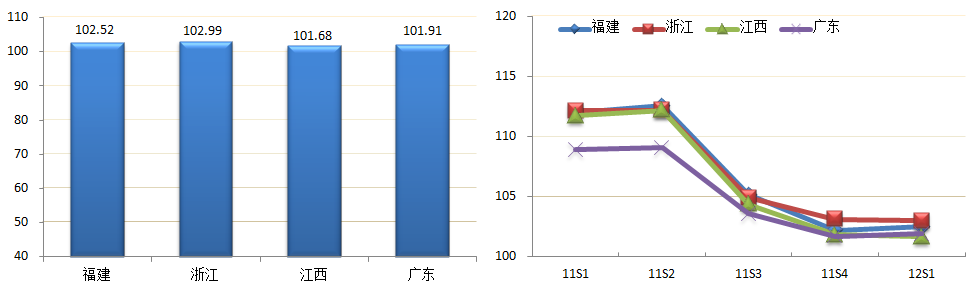
\includegraphics[width=16cm]{figure/各省生活状况信心指数}
\par\end{centering}

\centering{}\caption{\label{fig:=005404=007701=00751F=006D3B=0072B6=0051B5=004FE1=005FC3=006307=006570}各省生活状况信心指数}
\end{figure}



\subsubsection{就业信心评析}

图\ref{fig:=006D77=00897F=005C31=004E1A=004FE1=005FC3=006307=006570}显示,本季度海西地区就业信心指数为$91.00$,比上季度略升$0.10$点,与去年同期相比降低$7.25$点,落在悲观区域。海西地区民众对未来半年就业前景不甚乐观,主要有以下几方面原因:一是欧债危机持续发酵,美国对中国出口产品实施贸易制裁,使得海西地区大量出口和代工企业利润大幅降低;二是去年年底和今年年初东南沿海各地民间借贷资金链断裂,导致中小企业大量倒闭,大量进城务工人员返乡,与此同时$2012$年应届毕业生人数又创新高;三是国家发改委称“十二五”期间将重点整治水泥、钢铁等产能过剩行业,逐步淘汰落后产能。这些因素使民众对$2012$年上半年的就业形势比较悲观。
\begin{figure}[H]
\begin{centering}
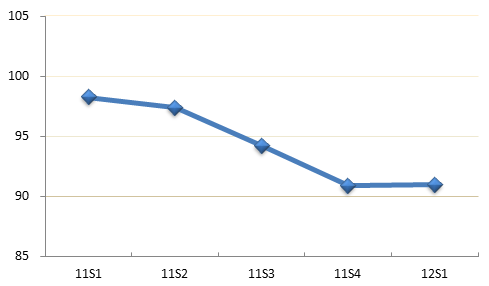
\includegraphics[width=9cm]{figure/海西就业信心指数}
\par\end{centering}

\centering{}\caption{\label{fig:=006D77=00897F=005C31=004E1A=004FE1=005FC3=006307=006570}海西就业信心指数}
\end{figure}


从分省数据来看,四省就业信心水平普遍较低,其中,最高的是福建,最低的是广东。值得注意的是,广东就业信心指数已经连续三个季度低于$90$,并且呈下降趋势,就业前景堪忧,如图\ref{fig:=005404=007701=005C31=004E1A=004FE1=005FC3=006307=006570}所示。
\begin{figure}[H]
\begin{centering}
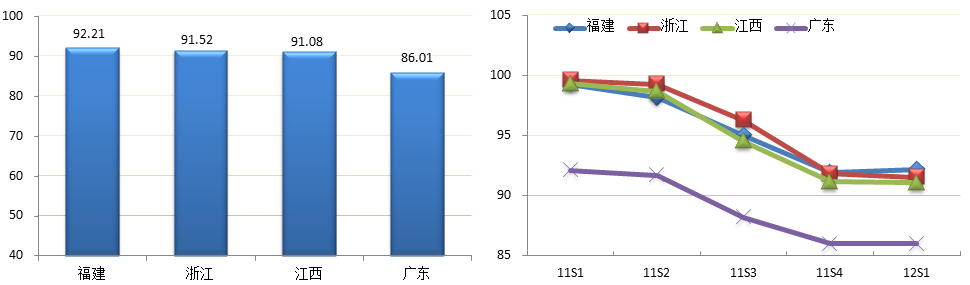
\includegraphics[width=16cm]{figure/各省就业信心指数}
\par\end{centering}

\centering{}\caption{\label{fig:=005404=007701=005C31=004E1A=004FE1=005FC3=006307=006570}各省就业信心指数}
\end{figure}



\subsubsection{耐用品消费及房地产购买信心评析}

本季度海西地区耐用品投资状况指数为$85.50$,处于悲观区域,比上季度回升$0.88$点,呈探底回升之势,同比下降$6.63$点。从分项指标来看,耐用品购买指数为$89.45$,环比上升$0.60$点,同比下降$8.25$点;房地产购买信心指数为$81.55$,环比上升$1.15$点,同比下降$5.00$点,如图\ref{fig:=006D77=00897F=008010=007528=0054C1=006295=008D44=004FE1=005FC3=006307=006570}所示。从耐用消费品方面来看,本季度央行两次下调存款准备金率,放宽的货币政策使耐用消费品回暖,但是通胀余威犹在,海西民众实际消费能力尚待提高。房地产调控政策已经实施一年有余,各城市房价尚未回归到合理水平,国家领导人在不同场合多次表示今年将继续实行房地产调控政策,因此虽然部分房地产开发商已经开始降价销售回笼资金,但是大部分海西民众对购买商品房依然持观望态度。
\begin{figure}[H]
\begin{centering}
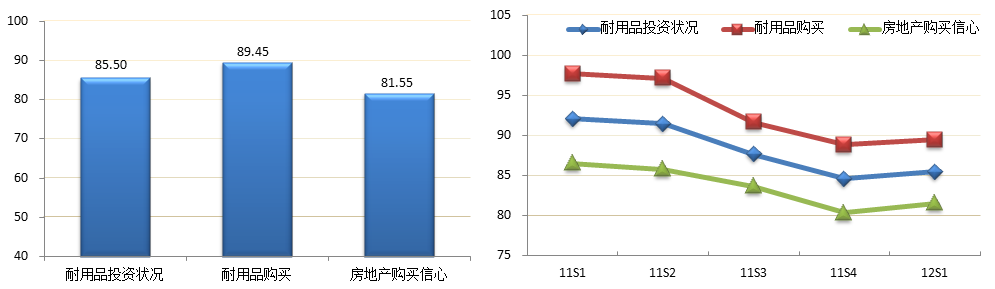
\includegraphics[width=16cm]{figure/海西耐用品投资信心指数}
\par\end{centering}

\centering{}\caption{\label{fig:=006D77=00897F=008010=007528=0054C1=006295=008D44=004FE1=005FC3=006307=006570}海西耐用品投资信心指数}
\end{figure}


海西各省的耐用品投资信心也较为低迷,情况相对较好的是浙江($87.12$),这与长三角地区强大的资金实力和区位优势密切相关,信心水平最低的是广东($82.30$),福建、江西处于中游水平,如图\ref{fig:=005404=007701=008010=007528=0054C1=006295=008D44=004FE1=005FC3=006307=006570}所示。
\begin{figure}[H]
\begin{centering}
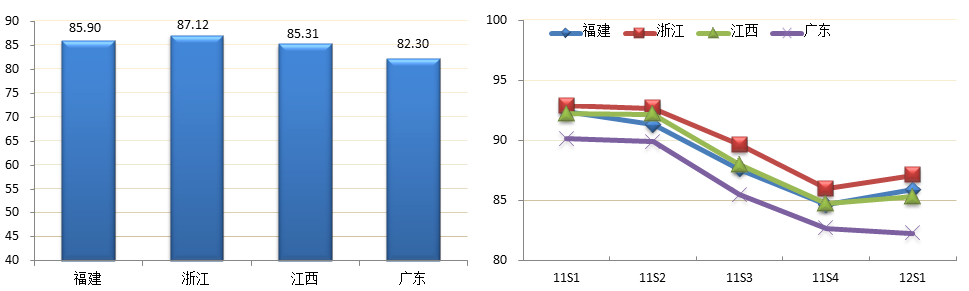
\includegraphics[width=16cm]{figure/各省耐用品投资信心指数}
\par\end{centering}

\centering{}\caption{\label{fig:=005404=007701=008010=007528=0054C1=006295=008D44=004FE1=005FC3=006307=006570}各省耐用品投资信心指数}
\end{figure}



\subsubsection{海西建设信心指数评析}

一季度海西建设信心指数是$98.00$,环比上升$0.10$点,同比下降$10.70$点,仍旧处于略微悲观区域。如图\ref{fig:=006D77=00897F=005EFA=008BBE=004FE1=005FC3=006307=006570}所示,继上季度该指数($97.90$)两年来首次跌入悲观区域之后,本季度指数有所回升,海西民众对未来半年海西地区建设的信心正在恢复。
\begin{figure}[H]
\begin{centering}
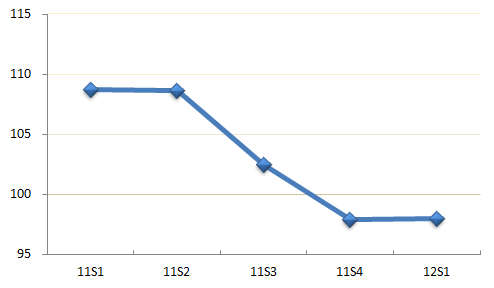
\includegraphics[width=9cm]{figure/海西建设信心指数}
\par\end{centering}

\centering{}\caption{\label{fig:=006D77=00897F=005EFA=008BBE=004FE1=005FC3=006307=006570}海西建设信心指数}
\end{figure}


如图\ref{fig:=005404=007701=006D77=00897F=005EFA=008BBE=004FE1=005FC3=006307=006570}所示,四省居民对未来半年海西建设信心略显不足,信心最高的是江西($99.67$),其次是广东($99.24$),福建($97.50$)、浙江($97.11$)分居第三和第四位。
\begin{figure}[H]
\begin{centering}
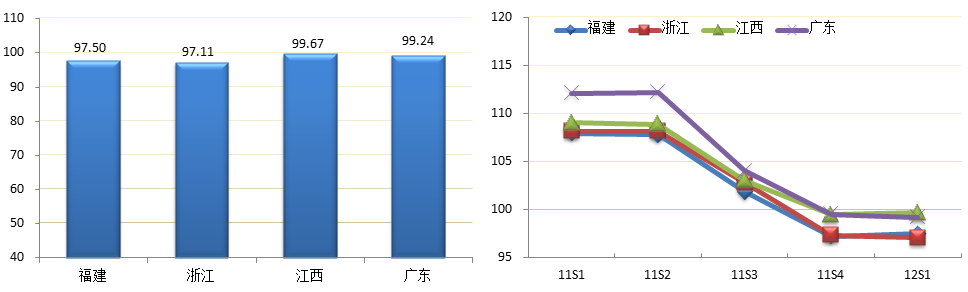
\includegraphics[width=16cm]{figure/各省海西建设信心指数}
\par\end{centering}

\centering{}\caption{\label{fig:=005404=007701=006D77=00897F=005EFA=008BBE=004FE1=005FC3=006307=006570}各省海西建设信心指数}
\end{figure}



\subsubsection{旅游信心指数评析}

本季度海西旅游信心指数较上一季度略下降$0.42$点,达到$110.18$,同比上升$7.55$点,如图\ref{fig:=006D77=00897F=0065C5=006E38=006307=006570}所示。对比过去一年数据,海西旅游信心指数从去年年初的$102.63$,稳步发展至今年一季度的$110.18$,每一季度增幅虽不迅猛,但整体趋势较为稳定,依旧保持乐观的发展倾向。从分项指标来看,旅游计划与旅游收入两项发展均衡,其中旅游计划$111.95$,旅游收入$108.40$,表明海西居民既有较强的出行意愿,愿意为休闲旅游支付成本,同时也对本地旅游收入持有信心,是一个很好的良性循环。

\begin{figure}[H]
\begin{centering}
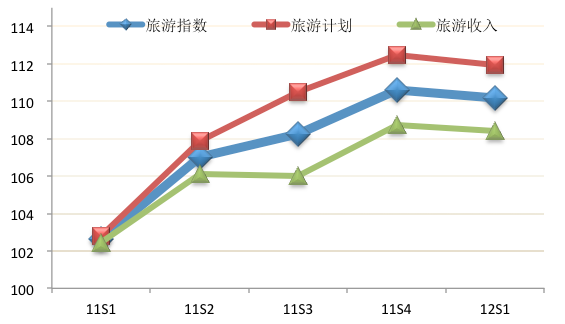
\includegraphics[width=9cm]{figure/海西旅游指数}
\par\end{centering}

\caption{\label{fig:=006D77=00897F=0065C5=006E38=006307=006570}海西旅游指数}
\end{figure}


随着国内各级地方政府“十二五”旅游业规划编制工作的完成,“十二五”期间将是我国建设为世界旅游强国的关键时期。近年来国人收入水平日渐提高,休闲观念逐步成熟,旅游消费日益成为大众选择;而高铁公里数的延伸、国家路网的贯通以及民航交通等基础设施的建设完善进一步刺激了广大居民的出行意愿;同时,各地地方政府越来越重视打造“城市名片”,挖掘本地特色旅游资源,完善旅游景区配套设施,旅游目的地选择愈发多样,丰富的旅游经历成为最好的宣传材料。$2012$年第一季度旅游信心指数的乐观度是今后旅游业良性发展的基石,旅游业以及由旅游业带动的相关产业,将成为国民经济的一项重要支柱。

旅游信心包括两大部分:旅游计划和旅游收入。从旅游计划方面来看,如图\ref{fig:=005404=007701=0065C5=006E38=008BA1=005212}所示,$2012$年第一季度海西福建、浙江、江西三省消费者评分皆在百分以上,持较为积极态度,出行意愿比较强烈;而广东省则继续维持低迷状态,仅为$88.23$。旅游收入信心方面与旅游计划较为相似,如图\ref{fig:=005404=007701=0065C5=006E38=006536=005165}所示,福建、浙江、江西三省继续持乐观态度,来自广州的被调查者则相对悲观,分值落差较大。这一情况与四省各自具有的旅游资源密切相关。福建的武夷山、厦门,浙江的雁荡山、大陈岛、横店影视城,江西的婺源、三清山、大觉山等均为全国知名旅游胜地,具有得天独厚的自然人文条件,且全省旅游资源丰富,连动效应明显;相较之下,广东省作为旅游目的地尚缺乏特定吸引力。而根据第六次人口普查数据,广东省流动人口占全省人口比例高达$20\%$以上,这部分人群的出行意愿和收入预期相对较为欠缺,也对广东省整体数据的低迷产生一定影响。 

对比以往数据,四省旅游计划和旅游收入信心对比上一季度均有不同程度的下降,如图\ref{fig:=005404=007701=0065C5=006E38=008BA1=005212}、图\ref{fig:=005404=007701=0065C5=006E38=006536=005165}折线图所示,而相较$2011$年第一季度,则获得较大提升。一方面,上一季度调查数据契合传统春节旅游旺季和春季旅游最佳时期,正值出行计划制定期,本季度略有微度下降实属合理区间;一方面,经过一年时间的培养,国人休闲度假习惯更加成熟,而浙江境内动车线路的丰富,龙厦高铁、龙深高铁贯通时间表的明晰,均为本地居民出行和旅游市场的兴旺提供了有利保障。随着国内经济走势日趋明朗,从大趋势上看,无论是旅游计划还是旅游收入,均将继续保持良性发展态势。

\begin{figure}[H]
\begin{centering}
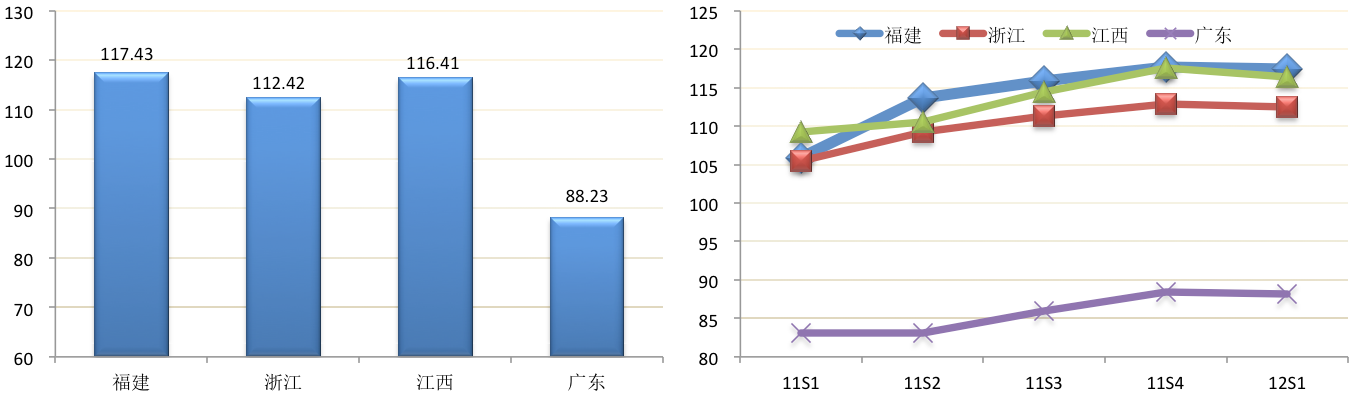
\includegraphics[width=16cm]{figure/各省旅游计划}
\par\end{centering}

\caption{\label{fig:=005404=007701=0065C5=006E38=008BA1=005212}各省旅游计划}
\end{figure}


\begin{figure}[H]
\begin{centering}
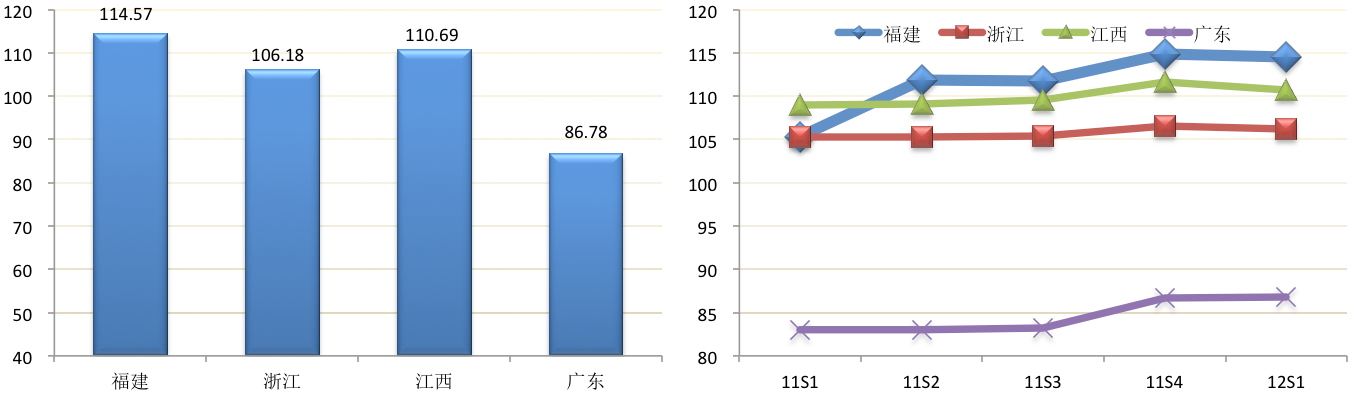
\includegraphics[width=16cm]{figure/各省旅游收入}
\par\end{centering}

\caption{\label{fig:=005404=007701=0065C5=006E38=006536=005165}各省旅游收入}
\end{figure}



\subsubsection{金融投资信心指数评析}

$2012$年第一季度海西地区金融指数为$69.03$,环比上升$2.78$点,同比略下降$0.70$点。从分省数据来看,浙江位居首位,指数达到$70.30$,福建为$69.89$,江西为$67.64$,广东则以$65.56$位居末位,福建环比增幅最大。从分项指数来看,海西金融投资计划指数和投资比例指数分别为$62.10$和$75.95$,金融投资计划指数环比增幅达到$4.30$点,为所有分项指数增幅最大值。

对比各季度总指数、消费指数、旅游指数和金融指数,如图\ref{fig:=005404=005B63=005EA6=006D77=00897F=006307=006570=003001=006D88=008D39=006307=006570=003001=0065C5=006E38=006307=006570=003001=0091D1=00878D=006307=006570}所示,三大指数中唯有金融指数与海西总指数整体波动方向一致,同增同减,相对于总指数的波动,海西指数波动明显扩大。由此可见,相对于消费指数和旅游指数,海西消费者金融信心水平的变动情况更充分反映了总体信心水平的变动情况,同时,本季度金融指数回调是海西整体信心指数上涨的主要推力。 

\begin{figure}[H]
\begin{centering}
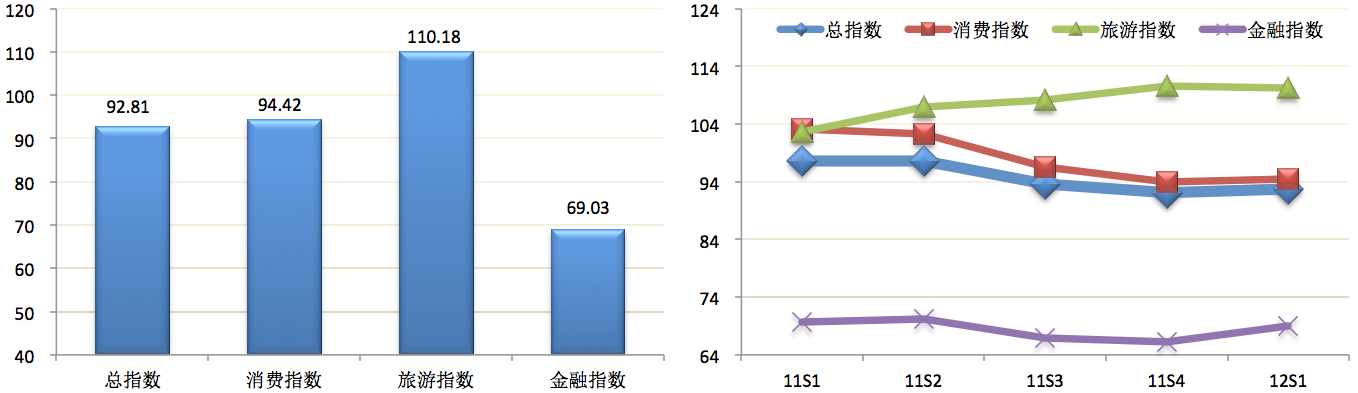
\includegraphics[width=16cm]{figure/各季度海西指数、消费指数、旅游指数、金融指数}
\par\end{centering}

\caption{\label{fig:=005404=005B63=005EA6=006D77=00897F=006307=006570=003001=006D88=008D39=006307=006570=003001=0065C5=006E38=006307=006570=003001=0091D1=00878D=006307=006570}各季度海西指数、消费指数、旅游指数、金融指数}
\end{figure}


本季度海西消费者金融投资信心有所回升,指数值触底回调,略改$2010$年开始调查海西指数以来震荡下滑的疲态,如图\ref{fig:=006D77=00897F=0091D1=00878D=006307=006570}所示。自$2010$年以来,宏观金融市场不景气,因此海西金融投资信心指数一直处于地位徘徊,随着$2012$年初货币政策放松预期以及中国股市反弹,海西消费者对金融投资的信心有所改善。

\begin{figure}[H]
\begin{centering}
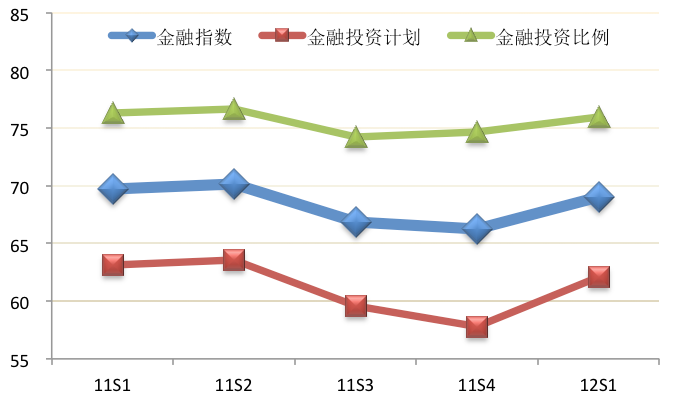
\includegraphics[width=9cm]{figure/海西金融指数}
\par\end{centering}

\caption{\label{fig:=006D77=00897F=0091D1=00878D=006307=006570}海西金融指数}
\end{figure}


从分项指数来看,本季度金融投资计划指数是所有分项指数环比增幅最大的指数值,表明海西消费者更愿意参与金融投资活动。受存款准备金率再次下调以及银行资金面进一步宽松的影响,海西消费者对海西未来半年内金融投资环境的信心有所改观。保险、证券等外资金融机构纷纷涉足海西证券市场,外资金融机构抢滩海西地区,从机构投资者的专业角度再次验证了海西金融环境不断上升的吸引力。

从分省数据来看,如图\ref{fig:=005404=007701=0091D1=00878D=006307=006570}所示,福建消费者金融投资信心改观最大,而正处于民间借贷风暴中心的浙江消费者金融投资信心依然高于海西其他地区,同时广东金融信心指数依然处于末位。究其原因,除海西金融行业本季度迎来众多的利好消息外,福建于$3$月中旬也出台支持金融行业发展的$9$条措施,政府政策的支持在民众心中起到了较大的作用。而浙江地区民间资本的富余促使当地消费者更倾向于灵活多样的金融投资,温州金融综合改革试验区的建立将为海西乃至全国民间金融的阳光化、规范化树立风向标,因此,浙江消费者金融投资意愿高于海西平均水平。然而,温州金融综合改革实验区的成功与否及其影响作用还有待时间的进一步考验。此外,以外向型经济为主导的广东深受全球性金融危机的影响,金融投资意愿明显低于海西其他地区。金融行业的发展问题是值得当地政府探讨的。首届岭南论坛众多金融业内人士指出,正值痛苦转型期的金融行业应该多管齐下来服务实体经济,这同样也是广东乃至海西金融行业未来的重要发展机遇。

\begin{figure}[H]
\begin{centering}
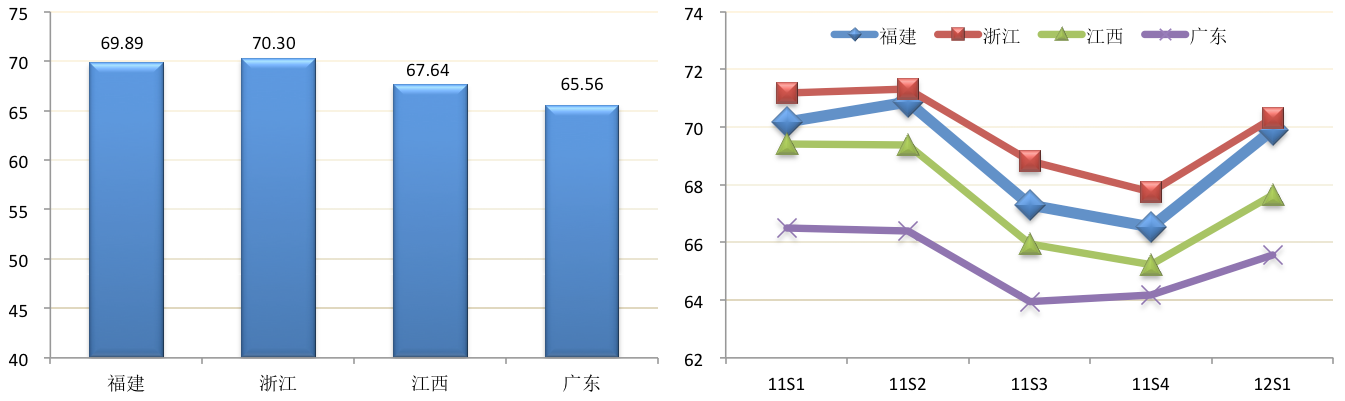
\includegraphics[width=16cm]{figure/各省金融指数}
\par\end{centering}

\caption{\label{fig:=005404=007701=0091D1=00878D=006307=006570}各省金融指数}
\end{figure}



\subsection{海峡两岸信心评析}

台湾方面,一季度物价水平指数为$56.97$,超过$50\%$的被调查者认为未来半年内物价会上涨;经济景气指数为$83.70$,说明台湾人民对未来半年的经济景气程度略显悲观。台湾的调查结果显示,未来半年家庭经济状况指数为$82.88$,欧债危机持续发酵、经济增速放缓和通胀高企已经影响到台湾人民的家庭生活。台湾就业信心指数为$105.13$,偏向乐观。$2012$年马英九在台湾大选中成功连任台湾地区领导人,宣布未来将重视分配和青年就业,使台湾民众对未来就业前景充满信心。台湾未来半年购买耐久性财货时机指数为$91.85$,未来半年投资股票时机指数为58.53,均落入悲观区域。

海峡两岸同根同源,随着近年来两岸在光电产业、精密仪器、金融服务和农副产品等产业上经济贸易合作交流的不断加深,海峡两岸信心指数走向逐渐趋于一致,同样面对着通货膨胀、经济增速放缓、耐用品消费及金融投资信心不足等挑战。海峡两岸充分利用经济发展水平、产业结构和人口结构等方面的优势互补,必将使合作双方取得双赢。

\newpage{}


\section{2012年第一季度厦门金融、旅游、消费信心指数调查报告}


\subsection{厦门指数综述}

本季度厦门总指数值为$93.28$,比上季度上升$0.71$点,比去年同期下降$4.96$点。其中消费指数是$93.38$,环比上升$0.65$点,同比下降$10.03$点;旅游指数是$117.46$,环比上升$0.10$点,同比大幅上升$11.91$点;金融指数是$68.72$,环比略升$1.56$点,同比降低$1.53$点。可以看出,旅游指数的同比大幅上升使总指数同比下降的幅度较小。


\subsection{厦门分项指数分析}


\subsubsection{经济发展信心评析}

图\ref{fig:=0053A6=0095E8=007ECF=006D4E=0053D1=005C55=004FE1=005FC3=006307=006570}显示,厦门经济发展指数$90.84$,环比上升$1.04$点,同比下降$15.01$点,环比升幅和同比降幅均大于海西地区。从分项指数来看,厦门物价指数$75.40$,环比上升$2.02$点,同比降低$15.01$点,说明厦门物价水平与整个海西地区相比还是偏高;经济景气指数$106.29$,环比略升$0.06$点,同比下降$15.02$点。厦门经济发展在整个海西地区处于领先水平,受区位优势和政策优惠的影响,前期发展较快,复苏动力也较强。但是从指数绝对数值来看,这种增长的优势正在逐渐减弱,需要寻找新的发展动力。

\begin{figure}[H]
\begin{centering}
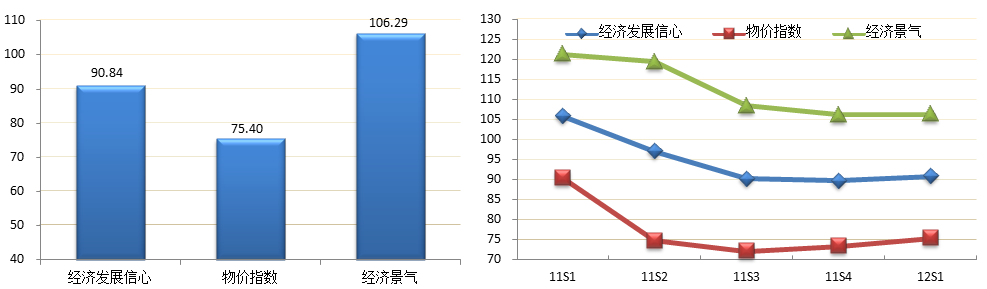
\includegraphics[width=16cm]{figure/厦门经济发展信心指数}
\par\end{centering}

\centering{}\caption{\label{fig:=0053A6=0095E8=007ECF=006D4E=0053D1=005C55=004FE1=005FC3=006307=006570}厦门经济发展信心指数}
\end{figure}



\subsubsection{家庭生活状况信心评析}

厦门一季度生活状况指数$102.50$,略高于海西地区水平,环比上升$0.30$点,同比降低$9.20$点。家庭经济状况指数$98.95$,环比上升$0.60$点,同比下降$11.51$点;家庭支出状况指数$106.06$,环比下降$0.01$点,同比下降$6.90$点,如图\ref{fig:=0053A6=0095E8=00751F=006D3B=0072B6=0051B5=004FE1=005FC3=006307=006570}所示。从指标值来看,厦门居民对未来半年生活状况的乐观程度略高于海西地区水平,但由于厦门物价较高,厦门家庭经济状况指数略低。

\begin{figure}[H]
\begin{centering}
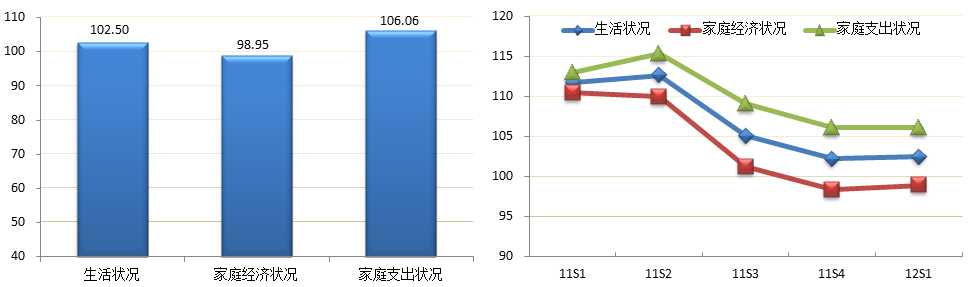
\includegraphics[width=16cm]{figure/厦门生活状况信心指数}
\par\end{centering}

\centering{}\caption{\label{fig:=0053A6=0095E8=00751F=006D3B=0072B6=0051B5=004FE1=005FC3=006307=006570}厦门生活状况信心指数}
\end{figure}



\subsubsection{就业信心指数}

如图\ref{fig:=0053A6=0095E8=005C31=004E1A=004FE1=005FC3=006307=006570}所示,厦门就业信心指数为$91.31$,比上季度上升$0.20$点,比去年同期下降$8.04$点,仍处于悲观区域,但悲观程度轻于全海西地区,这和厦门产业结构较为合理、作为经济特区和对台开放口岸有较多就业机会密不可分。

\begin{figure}[H]
\begin{centering}
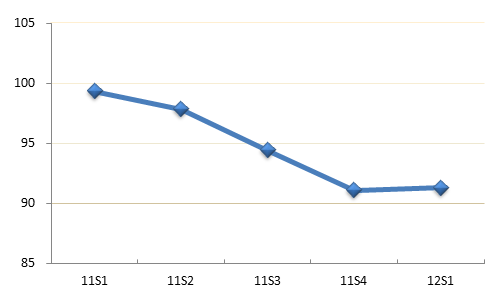
\includegraphics[width=9cm]{figure/厦门就业信心指数}
\par\end{centering}

\centering{}\caption{\label{fig:=0053A6=0095E8=005C31=004E1A=004FE1=005FC3=006307=006570}厦门就业信心指数}
\end{figure}



\subsubsection{耐用品消费信心及房地产购买信心评析}

厦门本季度耐用品投资状况指数为$85.57$,环比升高$1.14$点,同比降低$6.73$点。从分项指标来看,耐用品购买指数为$89.13$,环比上升$1.11$点,同比下降$8.63$点;房地产购买信心指数为$82.02$,环比上升$1.18$点,同比下降$4.83$点,详见图\ref{fig:=0053A6=0095E8=008010=007528=0054C1=006295=008D44=004FE1=005FC3=006307=006570}。虽然厦门耐用品购买指数略低于海西地区水平,但是房地产购买信心指数同比减少幅度相对较小,高于海西水平,这充分体现了厦门得天独厚的区位优势,资金与人流汇集,使厦门房地产降价速度相对较慢。

\begin{figure}[H]
\begin{centering}
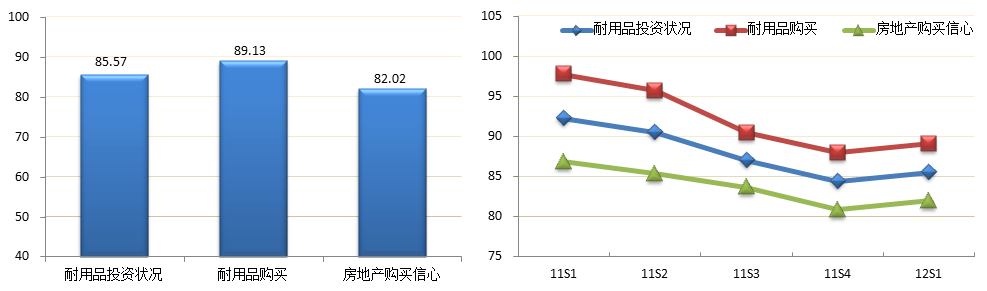
\includegraphics[width=16cm]{figure/厦门耐用品投资信心指数}
\par\end{centering}

\centering{}\caption{\label{fig:=0053A6=0095E8=008010=007528=0054C1=006295=008D44=004FE1=005FC3=006307=006570}厦门耐用品投资信心指数}
\end{figure}



\subsubsection{海西建设信心评析}

如图\ref{fig:=0053A6=0095E8=006D77=00897F=005EFA=008BBE=004FE1=005FC3=006307=006570}所示,厦门一季度海西建设信心指数是$97.90$,环比上升$0.02$点,同比下降$10.35$点,仍旧处于略微悲观区域。

\begin{figure}[H]
\centering{}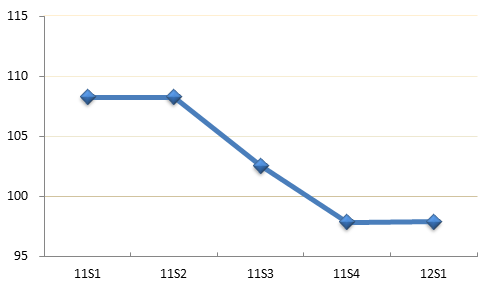
\includegraphics[width=9cm]{figure/厦门海西建设信心指数}\caption{\label{fig:=0053A6=0095E8=006D77=00897F=005EFA=008BBE=004FE1=005FC3=006307=006570}厦门海西建设信心指数}
\end{figure}



\subsubsection{旅游信心评析}

$2012$年第一季度调查结果显示,如图\ref{fig:=0053A6=0095E8=0065C5=006E38=006307=006570}所示,厦门旅游业发展态势稳中有升。从数据上看,该季度厦门旅游信心指数达到$117.46$,同比大涨$11.91$点,环比微升$0.10$点。在细分项目方面,厦门消费者旅游计划和旅游收入预期基本相当。其中,旅游计划指数$117.13$,同比上升$11.43$点,环比上升$0.16$点;旅游收入同比增加值较大,上涨$12.40$点,达到$117.80$,趋势更加乐观,环比略微上升$0.04$点。本地居民既有较强的出行愿望,也对厦门旅游市场充满信心。

在2011年厦门暂住人员赴金门一日游和厦门居民赴台个人游两大政策利好刺激下,厦门比邻台湾的得天独厚的区位优势得到充分释放,进一步激发了本地居民的出行意愿;而厦门往返武夷山航线的增加、福厦高铁的开通,便捷的交通也巩固了厦门作为旅游中转城市的地位;除此之外,得益于旅游质量、公共服务等服务保障能力的提升,截止$2011$年末,来厦游客的满意度已跃居全国$50$个重点旅游城市第三位,而投诉处理满意度更是实现全国第一;与此同时,随着厦门文化产业的充实,这座城市不仅释放着优越的自然条件,其独特的文化环境也吸引着越来越多的游客前来品位。$2011$年厦门旅游业增加值占全市GDP比重超过$9\%$,正成为厦门市国民经济的支柱产业。随着春季、夏季黄金旅游期到来,人们的出行意愿日益复苏,厦门的独特吸引力将继续发挥。

\begin{figure}[H]
\begin{centering}
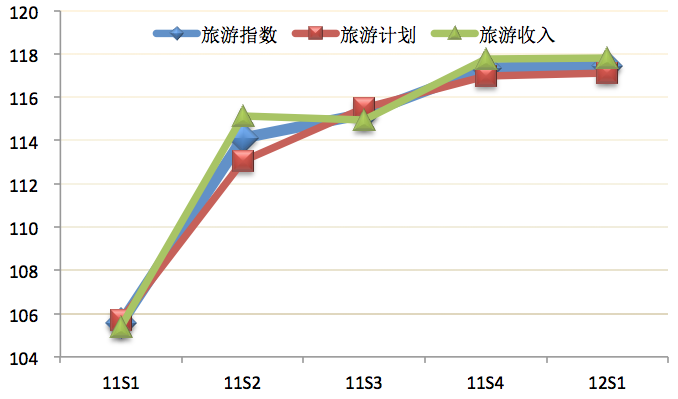
\includegraphics[width=9cm]{figure/厦门旅游指数}
\par\end{centering}

\caption{\label{fig:=0053A6=0095E8=0065C5=006E38=006307=006570}厦门旅游指数}
\end{figure}



\subsubsection{金融投资信心评析}

基于海西$2012$年第一季度金融行业的众多利好消息,厦门消费者金融投资信心有所改善,基本与海西消费者金融投资信心平均水平相持平,指数值达到$68.72$,环比上涨$1.56$点,同比略跌$1.53$点。

从分项指数来看,如图\ref{fig:=0053A6=0095E8=0091D1=00878D=006307=006570}所示,自$2010$年开始调查海西指数以来,厦门消费者金融投资的参与度均低于海西平均水平,但是一旦厦门消费者决定投资,其投资比例将高于海西平均水平。本季度金融投资计划、金融投资比例回调的幅度均小于海西平均水平,可见厦门消费者金融投资信心的改善势头略低于海西平均水平。考虑到厦门金融行业制度较为规范,厦门金融指数自$2010$年第四季度以来一直高于海西平均水平,即使本季度金融指数回调较小,但也与海西平均水平相持平。此外,除了本季度海西金融行业的整体影响因素以外,虽然本季度厦门获批可经营新台币兑换的银行增至7家,平潭对台综合实验区的成立可能对厦门产生了一定的冲击。厦门应继续充分发挥对台金融工作区位优势,推动深化两岸交流合作综合配套改革试验,提升自身竞争优势,方能进一步改善众多消费者的投资信心。

\begin{figure}[H]
\begin{centering}
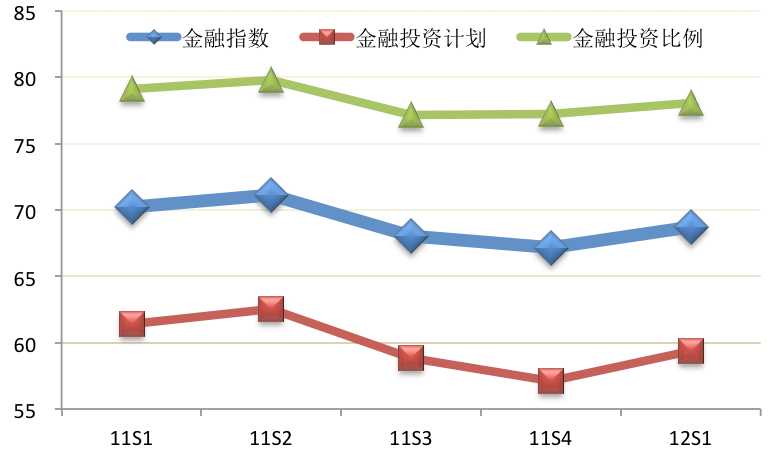
\includegraphics[width=9cm]{figure/厦门金融指数}
\par\end{centering}

\caption{\label{fig:=0053A6=0095E8=0091D1=00878D=006307=006570}厦门金融指数}
\end{figure}



\subsubsection{厦门信心指数与海西信心指数比较}

本季度厦门经济发展信心指数和金融指数低于海西地区水平。经济发展信心指数低于海西水平$4.46$点,主要是厦门物价水平偏高所致。金融指数低于海西水平$0.31$点,主要是本季度厦门金融投资计划、金融投资比例回调的幅度均小于海西平均水平。旅游指数依然是厦门的亮点,厦门旅游指数高于海西水平$7.29$点,在全海西地区旅游指数环比下降的情况厦门旅游指数环比增加。这几年厦门旅游持续升温,再加上“十二五”期间国家计划大力发展旅游业,旅游对厦门经济的贡献不可小觑。

\newpage{}


\section{结\quad 语}

纵观$2012$年第一季度海西金融、旅游、消费信心指数中各指数的表现,结合这些指数以往运行情况,一些趋势值得我们进一步关注:

第一,与去年同期相比,除旅游信心指数外,海西金融指数、消费指数均不及往年同期,且都落在不景气区域。应该说,海西金融、旅游、消费信心指数总体是不乐观的,居民对未来的预期远比去年同期谨慎,这是居民理性选择的表现,凸显出居民对未来经济发展有所信心不足,对未来经济环境看法总体较为保守。

第二,海西金融、旅游、消费信心指数中,除旅游指数微降外,其它分项指数环比均有所回升。$2011$年是转型之年,这一年除旅游指数之外,其他分项指数“满盘尽墨”,且各分项指数持续不乐观,呈现初步走低态势。如果说过去一年的海西是困惑的,那么新一期的指数则让我们感到了一丝春意。海西是否走出了“转型之惑”还值得进一步观察,但大部分指数出现回升,确实值得振奋。

第三,旅游指数在海西金融、旅游、消费信心指数中一枝独秀。旅游业是朝阳产业,是国家“促进消费”倡导产业,也是居民消费升级导向产业。海西旅游资源丰富,越来越多的人选择海西作为旅游目的地,也有越来越多海西居民选择外出旅游,以旅游来丰富家庭文化生活。从持续乐观的旅游指数看,海西应该打好旅游这张名片,以旅游促进区域经济发展,也以旅游拉动居民消费。

自金融危机以来,我国经济发展承受了多方面风险和挑战。在国际形势上,美国次贷危机刚刚过去,欧洲主权债务危机接踵而至,加之贸易摩擦和人民币汇率争议,复杂的国际环境给我国的出口、金融和货币政策带来了前所未有的冲击;在国内环境上,经历了三十多年高增长的中国,如何稳步实现经济结构调整,科学处理“好”与“快”的关系,破解发展中不平衡、不协调、不可持续的问题,都是摆在我们面前不得不解决的新情况。“转型和发展”是“十二五”规划的主体,在新的发展机遇期,是否做好准备迎接挑战,还有待我们进一步观察海西信心指数。


\section*{\newpage{}}


\section{附表:2012年第一季度总指数和各分项指数}

\begin{table}[H]
\begin{doublespace}
\caption{海西金融、旅游、消费信心指数}

\end{doublespace}

\centering{}{\footnotesize }%
\begin{tabular}{cr@{\extracolsep{0pt}.}lr@{\extracolsep{0pt}.}lr@{\extracolsep{0pt}.}lr@{\extracolsep{0pt}.}lccc}
\hline 
项 & \multicolumn{2}{c}{{\footnotesize 2010年}} & \multicolumn{2}{c}{{\footnotesize 2010年}} & \multicolumn{2}{c}{{\footnotesize 2011年}} & \multicolumn{2}{c}{{\footnotesize 2011年}} & {\footnotesize 2011年} & {\footnotesize 2011年} & {\footnotesize 2012年}\tabularnewline
目 & \multicolumn{2}{c}{{\footnotesize 第三季度}} & \multicolumn{2}{c}{{\footnotesize 第四季度}} & \multicolumn{2}{c}{{\footnotesize 第一季度}} & \multicolumn{2}{c}{{\footnotesize 第二季度}} & {\footnotesize 第三季度} & {\footnotesize 第四季度} & {\footnotesize 第一季度}\tabularnewline
\hline 
\textbf{总指数} & 98&01 & 101&48 & 97&54 & 97&66 & 93.53  & 92.11 & 92.81\tabularnewline
\hline 
\textbf{一、消费指数} & 103&18 & 105&16 & 103&22 & 102&21 & 96.50  & 93.96 & 94.42\tabularnewline
{\footnotesize 1、 经济发展信心} & 105&70 & 107&75  & 105&70 &  102&45 & 95.18 & 94.55 & 95.30\tabularnewline
{\footnotesize 物价指数} & 97&20 & 93&50 & 92&10 &  86&55 & 83.80 & 84.50 & 85.95\tabularnewline
{\footnotesize 经济景气} & 114&20  & 122&00  & 119&30  & 118&35 & 106.55 & 104.60 & 104.65\tabularnewline
{\footnotesize 2、生活状况} & 110&50 & 113&75  & 111&58  & 111&90 & 104.78  & 102.25 & 102.38\tabularnewline
{\footnotesize 家庭经济状况} & 110&95  & 113&40 & 110&30 &  109&90 & 102.05 & 99.50 & 99.85\tabularnewline
{\footnotesize 家庭支出状况} & 110&05 & 114&10  & 112&85  & 113&90 & 107.50 & 105.00 & 104.90\tabularnewline
{\footnotesize 3、就业信心指数} & 96&65 & 100&30 & 98&25  & 97&40 & 94.25  & 90.90 & 91.00\tabularnewline
{\footnotesize 4、耐用品投资状况} & 93&08  & 94&28  & 92&13  & 91&48 & 87.68  & 84.63 & 85.50\tabularnewline
{\footnotesize 耐用品购买} & 98&05  & 99&95  & 97&70 &  97&15 & 91.65  & 88.85 & 89.45\tabularnewline
{\footnotesize 房地产购买信心} & 88&10  & 88&60  & 86&55 &  85&80 & 83.70 & 80.40 & 81.55\tabularnewline
{\footnotesize 5、海西建设信心} & 110&25  & 109&45  & 108&70  & 108&65 & 102.50 & 97.90 & 98.00\tabularnewline
\hline 
\textbf{二、旅游指数} & 106&20 & 116&58 & 102&63  &  107&00 & 108.25  & 110.60 & 110.18\tabularnewline
{\footnotesize 1、旅游计划} & 88&45  & 100&60  & 102&80  & 107&90 & 110.50  & 112.45 & 111.95\tabularnewline
{\footnotesize 2、旅游收入} & 123&95  & 132&55  & 102&45 &  106&10 & 106.00 & 108.75 & 108.40\tabularnewline
\hline 
\textbf{三、金融指数} & 69&15  & 71&65 & 69&73  & 70&13 & 66.90 & 66.25 & 69.03\tabularnewline
{\footnotesize 1、金融投资计划} & 68&65 & 64&90  & 63&15  & 63&60  & 59.60 & 57.80 & 62.10\tabularnewline
{\footnotesize 2、金融投资比例} & 69&65  & 78&40  & 76&30  & 76&65 &  74.20 & 74.70 & 75.95\tabularnewline
\hline 
\end{tabular}
\end{table}


\newpage{}

\begin{table}[H]
\begin{doublespace}
\caption{福建省金融、旅游、消费信心指数}

\end{doublespace}

\centering{}{\footnotesize }%
\begin{tabular}{cr@{\extracolsep{0pt}.}lr@{\extracolsep{0pt}.}lr@{\extracolsep{0pt}.}lr@{\extracolsep{0pt}.}lccc}
\hline 
项 & \multicolumn{2}{c}{{\footnotesize 2010年}} & \multicolumn{2}{c}{{\footnotesize 2010年}} & \multicolumn{2}{c}{{\footnotesize 2011年}} & \multicolumn{2}{c}{{\footnotesize 2011年}} & {\footnotesize 2011年} & {\footnotesize 2011年} & {\footnotesize 2012年}\tabularnewline
目 & \multicolumn{2}{c}{{\footnotesize 第三季度}} & \multicolumn{2}{c}{{\footnotesize 第四季度}} & \multicolumn{2}{c}{{\footnotesize 第一季度}} & \multicolumn{2}{c}{{\footnotesize 第二季度}} & {\footnotesize 第三季度} & {\footnotesize 第四季度} & {\footnotesize 第一季度}\tabularnewline
\hline 
\textbf{总指数} & 99&50  & 102&34 & 98&37  & 98&52  & 94.25 & 92.79 & 93.82\tabularnewline
\hline 
\textbf{一、消费指数} & 104&16  & 105&63  & 103&60 & 101&88  & 96.10 & 93.48 & 94.26\tabularnewline
{\footnotesize 1、 经济发展信心} & 106&61  & 108&40  & 106&37  & 100&71  & 93.19 & 92.48 & 93.76\tabularnewline
{\footnotesize 物价指数} & 97&07  & 92&94  & 91&50  & 81&58  & 79.05 & 79.61 & 82.11\tabularnewline
{\footnotesize 经济景气} & 116&16  & 123&85  & 121&24  & 119&84  & 107.32 & 105.35 & 105.42\tabularnewline
{\footnotesize 2、生活状况} & 110&80  & 114&30  & 112&01  & 112&55  & 105.14 & 102.20 & 102.52\tabularnewline
{\footnotesize 家庭经济状况} & 110&31  & 113&83  & 110&73  & 110&30  & 101.82 & 99.08 & 99.62\tabularnewline
{\footnotesize 家庭支出状况} & 111&29  & 114&78  & 113&30  & 114&79  & 108.46 & 105.32 & 105.42\tabularnewline
{\footnotesize 3、就业信心指数} & 99&54  & 101&49  & 99&27  & 98&12  & 95.04 & 91.94 & 92.21\tabularnewline
{\footnotesize 4、耐用品投资状况} & 94&62  & 94&70 & 92&40  & 91&30  & 87.60 & 84.66 & 85.90\tabularnewline
{\footnotesize 耐用品购买} & 98&93  & 100&43  & 97&88  & 96&68  & 91.20 & 88.68 & 89.73\tabularnewline
{\footnotesize 房地产购买信心} & 90&31  & 88&97  & 86&93  & 85&92  & 84.00 & 80.64 & 82.06\tabularnewline
{\footnotesize 5、海西建设信心} & 109&67  & 108&74  & 107&93  & 107&79  & 101.86 & 97.24 & 97.50\tabularnewline
\hline 
\textbf{二、旅游指数} & 111&22  & 119&31  & 105&63 & 112&72  & 113.82 & 116.30 & 116.00\tabularnewline
{\footnotesize 1、旅游计划} & 94&81 & 104&04  & 105&91  & 113&62  & 115.91  & 117.72 & 117.43\tabularnewline
{\footnotesize 2、旅游收入} & 127&64  & 134&59  & 105&34  & 111&83  & 111.74 & 114.89 & 114.57\tabularnewline
\hline 
\textbf{三、金融指数} & 69&11  & 72&20  & 70&19  & 70&88 &  67.29 & 66.53 & 69.89\tabularnewline
{\footnotesize 1、金融投资计划} & 65&07  & 63&57  & 61&83  & 62&66  & 58.30 & 56.40 & 61.18\tabularnewline
{\footnotesize 2、金融投资比例} & 73&15  & 80&82 & 78&56  & 79&09  & 76.28 & 76.66 & 78.59\tabularnewline
\hline 
\end{tabular}
\end{table}


\newpage{}

\begin{table}[H]
\begin{doublespace}
\caption{浙江金融、旅游、消费信心指数}

\end{doublespace}

\centering{}{\footnotesize }%
\begin{tabular}{cr@{\extracolsep{0pt}.}lr@{\extracolsep{0pt}.}lr@{\extracolsep{0pt}.}lr@{\extracolsep{0pt}.}lccc}
\hline 
项 & \multicolumn{2}{c}{{\footnotesize 2010年}} & \multicolumn{2}{c}{{\footnotesize 2010年}} & \multicolumn{2}{c}{{\footnotesize 2011年}} & \multicolumn{2}{c}{{\footnotesize 2011年}} & {\footnotesize 2011年} & {\footnotesize 2011年} & {\footnotesize 2012年}\tabularnewline
目 & \multicolumn{2}{c}{{\footnotesize 第三季度}} & \multicolumn{2}{c}{{\footnotesize 第四季度}} & \multicolumn{2}{c}{{\footnotesize 第一季度}} & \multicolumn{2}{c}{{\footnotesize 第二季度}} & {\footnotesize 第三季度} & {\footnotesize 第四季度} & {\footnotesize 第一季度}\tabularnewline
\hline 
\textbf{总指数} & 96&24  & 102&69  & 98&75  & 98&97  & 95.09 & 93.29 & 93.79\tabularnewline
\hline 
\textbf{一、消费指数} & 101&65  & 105&89  & 103&99  & 103&80  & 98.33 & 95.58 & 95.79\tabularnewline
{\footnotesize 1、 经济发展信心} & 104&61  & 109&26  & 107&09 & 106&65  & 99.24  & 98.60 & 98.72\tabularnewline
{\footnotesize 物价指数} & 98&04  & 93&82  & 92&30  & 92&24  & 89.63 & 90.56 & 90.86\tabularnewline
{\footnotesize 经济景气} & 111&19  & 124&70 & 121&89  & 121&05  & 108.84 & 106.65 & 106.57\tabularnewline
{\footnotesize 2、生活状况} & 109&13  & 114&32  & 112&13  & 112&18  & 104.89 & 103.13 & 102.99\tabularnewline
{\footnotesize 家庭经济状况} & 110&99  & 112&89  & 109&46  & 109&24  & 101.59 & 99.27 & 99.15\tabularnewline
{\footnotesize 家庭支出状况} & 107&26  & 115&74  & 114&80  & 115&11  & 108.18 & 106.98 & 106.83\tabularnewline
{\footnotesize 3、就业信心指数} & 92&94  & 101&70  & 99&59 & 99&26 &  96.28 & 91.82 & 91.52\tabularnewline
{\footnotesize 4、耐用品投资状况} & 91&39  & 94&71  & 92&87  & 92&68  & 89.66 & 86.00 & 87.12\tabularnewline
{\footnotesize 耐用品购买} & 96&88  & 100&14  & 98&71  & 98&78  & 94.22 & 91.22 & 91.46\tabularnewline
{\footnotesize 房地产购买信心} & 85&89  & 89&28  & 87&02  & 86&57  & 85.10 & 80.78 & 82.78\tabularnewline
{\footnotesize 5、海西建设信心} & 109&97  & 108&82  & 108&17  & 108&16 &  102.79 & 97.34 & 97.11\tabularnewline
\hline 
\textbf{二、旅游指数} & 99&73  & 119&57  & 105&34  & 107&29  & 108.38 & 109.68 & 109.30\tabularnewline
{\footnotesize 1、旅游计划} & 80&87  & 103&39  & 105&40  & 109&24  & 111.37 & 112.84 & 112.42\tabularnewline
{\footnotesize 2、旅游收入} & 118&59  & 135&75  & 105&27  & 105&33  & 105.39 & 106.52 & 106.18\tabularnewline
\hline 
\textbf{三、金融指数} & 71&10  & 73&00  & 71&18  & 71&32  & 68.82 & 67.75 & 70.30\tabularnewline
{\footnotesize 1、金融投资计划} & 74&01  & 63&97  & 62&03  & 62&14  & 58.84 & 56.31 & 61.10\tabularnewline
{\footnotesize 2、金融投资比例} & 68&18  & 82&02  & 80&33  & 80&50  & 78.79 & 79.19 & 79.50\tabularnewline
\hline 
\end{tabular}
\end{table}


\newpage{}

\begin{table}[H]
\begin{doublespace}
\caption{江西金融、旅游、消费信心指数}

\end{doublespace}

\centering{}{\footnotesize }%
\begin{tabular}{cr@{\extracolsep{0pt}.}lr@{\extracolsep{0pt}.}lr@{\extracolsep{0pt}.}lr@{\extracolsep{0pt}.}lccc}
\hline 
项 & \multicolumn{2}{c}{{\footnotesize 2010年}} & \multicolumn{2}{c}{{\footnotesize 2010年}} & \multicolumn{2}{c}{{\footnotesize 2011年}} & \multicolumn{2}{c}{{\footnotesize 2011年}} & {\footnotesize 2011年} & {\footnotesize 2011年} & {\footnotesize 2012年}\tabularnewline
目 & \multicolumn{2}{c}{{\footnotesize 第三季度}} & \multicolumn{2}{c}{{\footnotesize 第四季度}} & \multicolumn{2}{c}{{\footnotesize 第一季度}} & \multicolumn{2}{c}{{\footnotesize 第二季度}} & {\footnotesize 第三季度} & {\footnotesize 第四季度} & {\footnotesize 第一季度}\tabularnewline
\hline 
\textbf{总指数} & 96&58 & 102&08  & 98&57  & 98&57  & 94.24 & 92.79 & 93.03\tabularnewline
\hline 
\textbf{一、消费指数} & 102&24  & 105&18 & 103&22  & 103&05  & 96.87 & 94.23 & 94.25\tabularnewline
{\footnotesize 1、 经济发展信心} & 104&61  & 109&26  & 107&09 & 106&65  & 99.24  & 95.03 & 94.65\tabularnewline
{\footnotesize 物价指数} & 95&26  & 91&14  & 90&18  & 88&66  & 86.20 & 86.20 & 85.60\tabularnewline
{\footnotesize 经济景气} & 113&86  & 122&37  & 119&30  & 119&46  & 106.43 & 103.86 & 103.70\tabularnewline
{\footnotesize 2、生活状况} & 111&31  & 113&90  & 111&75  & 112&17  & 104.37 & 101.84 & 101.68\tabularnewline
{\footnotesize 家庭经济状况} & 114&21  & 115&08  & 111&93  & 112&13  & 102.40 & 100.00 & 100.08\tabularnewline
{\footnotesize 家庭支出状况} & 108&42  & 112&72  & 111&58  & 112&22  & 106.35 & 103.69 & 103.28\tabularnewline
{\footnotesize 3、就业信心指数} & 94&91  & 101&84  & 99&30  & 98&69  & 94.51 & 91.17 & 91.08\tabularnewline
{\footnotesize 4、耐用品投资状况} & 90&35  & 94&38  & 92&24  & 92&19  & 87.99 & 84.73 & 85.31\tabularnewline
{\footnotesize 耐用品购买} & 96&22  & 100&52  & 97&89  & 97&91  & 92.20 & 87.91 & 88.21\tabularnewline
{\footnotesize 房地产购买信心} & 84&48  & 88&25  & 86&58  & 86&48  & 83.79 & 81.56 & 82.41\tabularnewline
{\footnotesize 5、海西建设信心} & 110&52  & 109&48  & 109&04  & 108&90  & 103.08 & 99.48 & 99.67\tabularnewline
\hline 
\textbf{二、旅游指数} & 101&88  & 120&00  & 109&08  & 109&82  & 112.01 & 114.58 & 113.55\tabularnewline
{\footnotesize 1、旅游计划} & 82&45  & 106&31  & 109&21  & 110&56 &  114.41 & 117.50 & 116.41\tabularnewline
{\footnotesize 2、旅游收入} & 121&31  & 133&68  & 108&95  & 109&07  & 109.60  & 111.66 & 110.69\tabularnewline
\hline 
\textbf{三、金融指数} & 68&64  & 71&80  & 69&43  & 69&37  & 65.95 & 65.23 & 67.64\tabularnewline
{\footnotesize 1、金融投资计划} & 71&84 & 63&42  & 62&19  & 61&87 &  57.38 & 55.67 & 59.35\tabularnewline
{\footnotesize 2、金融投资比例} & 65&44  & 80&18 & 76&67  & 76&88  & 74.53 & 74.79 & 75.93\tabularnewline
\hline 
\end{tabular}
\end{table}


\newpage{}

\begin{table}[H]
\begin{doublespace}
\caption{广东金融、旅游、消费信心指数}

\end{doublespace}

\centering{}{\footnotesize }%
\begin{tabular}{cr@{\extracolsep{0pt}.}lr@{\extracolsep{0pt}.}lr@{\extracolsep{0pt}.}lr@{\extracolsep{0pt}.}lccc}
\hline 
项 & \multicolumn{2}{c}{{\footnotesize 2010年}} & \multicolumn{2}{c}{{\footnotesize 2010年}} & \multicolumn{2}{c}{{\footnotesize 2011年}} & \multicolumn{2}{c}{{\footnotesize 2011年}} & {\footnotesize 2011年} & {\footnotesize 2011年} & {\footnotesize 2012年}\tabularnewline
目 & \multicolumn{2}{c}{{\footnotesize 第三季度}} & \multicolumn{2}{c}{{\footnotesize 第四季度}} & \multicolumn{2}{c}{{\footnotesize 第一季度}} & \multicolumn{2}{c}{{\footnotesize 第二季度}} & {\footnotesize 第三季度} & {\footnotesize 第四季度} & {\footnotesize 第一季度}\tabularnewline
\hline 
\textbf{总指数} & 96&08 & 96&40 & 92&23 & 92&15  & 88.35 & 87.57 & 87.89\tabularnewline
\hline 
\textbf{一、消费指数} & 102&40  & 102&64  & 100&95  & 100&86  & 95.39 & 93.43 & 93.58\tabularnewline
{\footnotesize 1、 经济发展信心} & 104&41 & 104&57 & 102&65 & 102&49 & 96.33 & 96.52 & 97.48\tabularnewline
{\footnotesize 物价指数} & 98&02 & 97&54 & 95&66 & 95&67  & 91.88 & 93.05 & 94.80\tabularnewline
{\footnotesize 经济景气} & 110&79  & 111&59  & 109&64  & 109&31  & 100.78 & 100.00 & 100.15\tabularnewline
{\footnotesize 2、生活状况} & 110&83  & 110&99  & 108&92  & 109&07  & 103.60 & 101.72 & 101.91\tabularnewline
{\footnotesize 家庭经济状况} & 110&87  & 110&71  & 108&37  & 107&80  & 102.81 & 100.86 & 100.84\tabularnewline
{\footnotesize 家庭支出状况} & 110&79 & 111&27  & 109&48  & 110&33  & 104.38 & 102.58 & 102.98\tabularnewline
{\footnotesize 3、就业信心指数} & 92&46  & 93&02  & 92&10  & 91&72  & 88.20 & 86.01 & 86.01\tabularnewline
{\footnotesize 4、耐用品投资状况} & 91&94  & 92&26  & 90&13  & 89&91  & 85.51 & 82.70 & 82.30\tabularnewline
{\footnotesize 耐用品购买} & 98&01  & 97&70  & 95&73  & 95&82  & 89.69 & 87.58 & 86.93\tabularnewline
{\footnotesize 房地产购买信心} & 85&87  & 86&82  & 84&52  & 83&99  & 81.33 & 77.81 & 77.67\tabularnewline
{\footnotesize 5、海西建设信心} & 112&38  & 112&46  & 112&08  & 112&22  & 104.07 & 99.53 & 99.24\tabularnewline
\hline 
\textbf{二、旅游指数} & 99&44 & 100&00  & 83&06  & 83&09  & 84.61 & 87.54 & 87.50\tabularnewline
{\footnotesize 1、旅游计划} & 79&60  & 80&24  & 83&10  & 83&13  & 86.01 & 88.43 & 88.23\tabularnewline
{\footnotesize 2、旅游收入} & 119&28  & 119&76  & 83&02  & 83&04  & 83.21 & 86.64 & 86.78\tabularnewline
\hline 
\textbf{三、金融指数} & 67&42  & 67&86  & 66&51  & 66&41  & 63.95 & 64.18 & 65.56\tabularnewline
{\footnotesize 1、金融投资计划} & 72&55  & 72&23  & 70&38  & 70&27  & 67.03 & 66.33 & 68.73\tabularnewline
{\footnotesize 2、金融投资比例} & 62&30  & 63&49  & 62&64  & 62&54  & 60.86 & 62.03 & 62.39\tabularnewline
\hline 
\end{tabular}
\end{table}


\newpage{}

\begin{table}[H]
\begin{doublespace}
\caption{厦门金融、旅游、消费信心指数(一)}

\end{doublespace}

\centering{}{\footnotesize }%
\begin{tabular}{cccccr@{\extracolsep{0pt}.}lr@{\extracolsep{0pt}.}lr@{\extracolsep{0pt}.}l}
\hline 
项 & {\footnotesize 2009年} & {\footnotesize 2009年} & {\footnotesize 2009年} & {\footnotesize 2009年} & \multicolumn{2}{c}{{\footnotesize 2010年}} & \multicolumn{2}{c}{{\footnotesize 2010年}} & \multicolumn{2}{c}{{\footnotesize 2010年}}\tabularnewline
目 & {\footnotesize 第一季度} & {\footnotesize 第二季度} & {\footnotesize 第三季度} & {\footnotesize 第四季度} & \multicolumn{2}{c}{{\footnotesize 第一季度}} & \multicolumn{2}{c}{{\footnotesize 第二季度}} & \multicolumn{2}{c}{{\footnotesize 第三季度}}\tabularnewline
\hline 
\textbf{总指数} & 94.06  & 94.57  & 97.00  & 100.85  & 109&15  & 104&58  & 101&53 \tabularnewline
\hline 
\textbf{一、消费指数} & 106.09  & 106.35  & 107.91  & 109.09  & 112&69  & 109&04  & 105&83 \tabularnewline
{\footnotesize 1、 经济发展信心} & — & — & — & — & 113&60 & 112&70  & 109&73 \tabularnewline
{\footnotesize 物价指数} & 115.85  & 117.80  & 119.95  & 114.45  & 103&60  & 101&10  & 98&80 \tabularnewline
{\footnotesize 经济景气} & — & — & — & — & 123&60 & 124&30  & 120&65 \tabularnewline
{\footnotesize 2、生活状况} & 101.75  & 101.50  & 101.73  & 103.60  & 118&90  & 120&25  & 112&23\tabularnewline
{\footnotesize 家庭经济状况} & 110.05  & 110.45 & 110.25 & 111.90  & 124&45 & 125&50  & 110&55 \tabularnewline
{\footnotesize 家庭支出状况} & 93.45  & 92.55  & 93.20  & 95.30  & 113&35  & 115&00  & 113&90 \tabularnewline
{\footnotesize 3、就业信心指数} & — & — & — & — & 110&00 & 104&20 & 104&15 \tabularnewline
{\footnotesize 4、耐用品投资状况} & 105.00  & 104.60  & 108.25  & 114.70 & 106&50  & 96&78 & 95&83\tabularnewline
{\footnotesize 耐用品购买} & — & — & — & — & 109&89  & 100&60  & 101&25\tabularnewline
{\footnotesize 房地产购买信心} & — & — & — & — & 103&11  & 92&95 & 90&40\tabularnewline
{\footnotesize 5、海西建设信心} & — & — & — & — & 113&55 & 108&65  & 106&95\tabularnewline
\hline 
\textbf{二、旅游指数} & 96.73  & 96.35 & 100.20 & 104.58 & 112&05 & 115&90  & 117&68 \tabularnewline
{\footnotesize 1、旅游计划} & 73.70  & 74.15 & 79.70  & 82.75  & 94&80  & 99&55 & 101&95\tabularnewline
{\footnotesize 2、旅游收入} & 119.75  & 118.55  & 120.70 & 126.40  & 129&30  & 132&25 & 133&40\tabularnewline
\hline 
\textbf{三、金融指数} & 67.33  & 69.23 & 71.98  & 80.65  & 92&10 & 75&40  & 68&20\tabularnewline
{\footnotesize 1、金融投资计划} & 52.00  & 57.40 & 62.50 & 69.00  & 82&30  & 57&30  & 57&50\tabularnewline
{\footnotesize 2、金融投资比例} & 82.65  & 81.05  & 81.45  & 92.30 & 101&90  & 93&50 & 78&90\tabularnewline
\hline 
\end{tabular}
\end{table}


\newpage{}

\begin{table}[H]
\begin{doublespace}
\caption{厦门金融、旅游、消费信心指数(二)}

\end{doublespace}

\centering{}{\footnotesize }%
\begin{tabular}{cr@{\extracolsep{0pt}.}lr@{\extracolsep{0pt}.}lr@{\extracolsep{0pt}.}lccc}
\hline 
项 & \multicolumn{2}{c}{{\footnotesize 2010年}} & \multicolumn{2}{c}{{\footnotesize 2011年}} & \multicolumn{2}{c}{{\footnotesize 2011年}} & {\footnotesize 2011年} & {\footnotesize 2011年} & {\footnotesize 2012年}\tabularnewline
目 & \multicolumn{2}{c}{{\footnotesize 第四季度}} & \multicolumn{2}{c}{{\footnotesize 第一季度}} & \multicolumn{2}{c}{{\footnotesize 第二季度}} & {\footnotesize 第三季度} & {\footnotesize 第四季度} & {\footnotesize 第一季度}\tabularnewline
\hline 
\textbf{总指数} & 102&21  & 98&24  & 98&10  & 94.04 & 92.57 & 93.28\tabularnewline
\hline 
\textbf{一、消费指数} & 105&53  & 103&41 & 100&84  & 95.25 & 92.73 & 93.38\tabularnewline
{\footnotesize 1、 经济发展信心} & 107&85  & 105&85  & 97&13  & 90.30 & 89.80 & 90.84\tabularnewline
{\footnotesize 物价指数} & 92&20  & 90&40  & 74&80  & 72.20 & 73.38 & 75.40\tabularnewline
{\footnotesize 经济景气} & 123&50  & 121&30  & 119&45  & 108.40 & 106.22 & 106.29\tabularnewline
{\footnotesize 2、生活状况} & 114&05  & 111&70  & 112&65  & 105.13 & 102.20 & 102.50\tabularnewline
{\footnotesize 家庭经济状况} & 113&55  & 110&45  & 109&95 &  101.20 & 98.34 & 98.95\tabularnewline
{\footnotesize 家庭支出状况} & 114&55 & 112&95 & 115&35  & 109.05 & 106.07 & 106.06\tabularnewline
{\footnotesize 3、就业信心指数} & 101&85  & 99&35  & 97&85 &  94.45 & 91.11 & 91.31\tabularnewline
{\footnotesize 4、耐用品投资状况} & 94&73 & 92&30  & 90&55 &  87.08 & 84.43 & 85.57\tabularnewline
{\footnotesize 耐用品购买} & 100&45  & 97&75  & 95&75  & 90.45 & 88.01 & 89.13\tabularnewline
{\footnotesize 房地产购买信心} & 89&00  & 86&85  & 85&35  & 83.70  & 80.85 & 82.02\tabularnewline
{\footnotesize 5、海西建设信心} & 109&10 & 108&25 & 108&25 &  102.55 & 97.89 & 97.90\tabularnewline
\hline 
\textbf{二、旅游指数} & 119&28 & 105&55 & 114&10  & 115.23 & 117.36 & 117.46\tabularnewline
{\footnotesize 1、旅游计划} & 103&85 & 105&70  & 113&05  & 115.50 & 116.97 & 117.13\tabularnewline
{\footnotesize 2、旅游收入} & 134&70  & 105&40 & 115&15 &  114.95 & 117.76 & 117.80\tabularnewline
\hline 
\textbf{三、金融指数} & 71&88  & 70&25  & 71&15  & 68.00 & 67.16 & 68.72\tabularnewline
{\footnotesize 1、金融投资计划} & 63&10  & 61&40  & 62&50  & 58.85 & 57.09 & 59.41\tabularnewline
{\footnotesize 2、金融投资比例} & 80&65  & 79&10  & 79&80  & 77.15 & 77.23 & 78.03\tabularnewline
\hline 
\end{tabular}
\end{table}


\newpage{}

\thispagestyle{empty}


\section*{北京商智通信息技术有限公司}


\subsection*{专注擅长领域,专业造就成功!}

\begin{center}
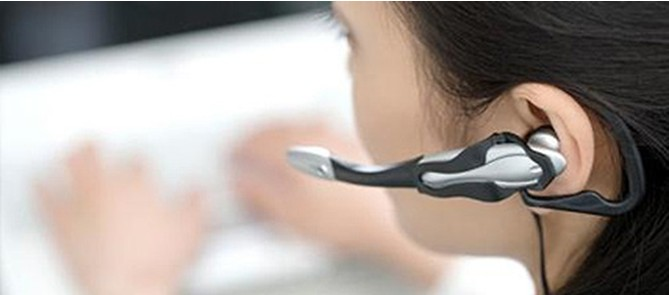
\includegraphics[width=12cm]{figure/szt}
\par\end{center}

北京商智通信息技术有限公司(\url{http://www.BIStone.com})是隶属于商智通集团( BIStone Group
) 的高新技术企业。公司致力于帮助企业“挖掘数据财富,开启商务智能”,为企业提供数量化管理软件和咨询服务,帮助企业获得“数量化管理能力”。

公司自成立以来,成功实施“榜样力量”与“战略联盟”两项战略。“榜样力量”战略方面:公司核心产品“TCSS 企业客户满意晴雨表”成功应用于物流、金融、保险、航空运输、制造业等标杆企业。而“战略联盟”方面:公司在咨询和管理软件两大领域分别寻找一家具有国际声誉与竞争优势的企业作为战略合作伙伴。“客户满意度”咨询方面与世界著名的标准认证咨询机构
BSI(英国标准协会)签署了排他性战略合作协议;文本挖掘、数量化管理培训方面与中华资料采矿协会达成知识管理、研发管理系列合作协议;数据挖掘、质量管理工具软件方面成为了统计领域工具软件领头企业——StatSoft(STATISTICA)在中国的销售、咨询、技术支持和培训合作伙伴;决策分析软件方面成为领先的决策支持工具软件商
Vangard Soft 在中国的合作伙伴。

商智通先后为政府、电力、电信、移动、网通、银行等国内企业提供专业的市场研究、客户满意度咨询、调查技术支持、数据挖掘咨询服务,积累了丰富的行业实战经验,得到广大客户的高度认可,同时赢得良好的信誉,为企业的持续发展打下了坚实的基础。公司在中国的典型客户有:中国远洋物流公司(TCSS
客户满意管理系统)、中国人民大学(TCSS金融业分析系统)、 BSI(英国标准协会)(TCSS 系统和客户满意咨询)、中国海关总暑(TCSS
进出口预测系统)、机械工业出版社(TCSS 图书数量化管理平台)、 ABB(中国)公司、中国检验检疫科学研究院等等。

商智通非常注重技术团队的培养、专业咨询团队的建设,荟萃了一批在海内外工作多年,拥有先进国际管理工作经验和丰富专业知识的咨询及研发人员,已经形成了具有深厚理论素养和实战管理咨询经验、良好的技术素养的程序开发人员、市场研究咨询师、调查技术咨询师和训练师的专业顾问团队。 
\end{document}
